\documentclass[listof= totoc]{scrreprt}
\usepackage[utf8]{inputenc}
\usepackage{lmodern}
\renewcommand*\familydefault{\sfdefault}
\usepackage[english]{babel}
\usepackage[T1]{fontenc}
\usepackage{booktabs}
\usepackage{amsfonts}
\usepackage{amsmath,hyperref}
\usepackage{amssymb}
\numberwithin{equation}{section}
\usepackage{braket}

\usepackage{siunitx} %Das ist für die Einheiten
\sisetup{
	locale = DE
}
\usepackage{graphicx}
\usepackage{epstopdf}
\usepackage{subfig}
\usepackage{tabulary}
\usepackage{float}
\usepackage{hpstatement}
\usepackage{multirow}
\usepackage{bm}
\usepackage{upgreek}
\usepackage{sansmathfonts}
\usepackage[left=2.5cm,right=2.5cm,top=2.5cm,bottom=2.5cm]{geometry}
\author{Gereon Feldmann}
\usepackage{setspace}
\usepackage{caption}
\makeatletter
\newcommand{\MSonehalfspacing}{%
	\setstretch{1.44}%  default
	\ifcase \@ptsize \relax % 10pt
	\setstretch {1.448}%
	\or % 11pt
	\setstretch {1.399}%
	\or % 12pt
	\setstretch {1.433}%
	\fi
}

\newcommand{\MSdoublespacing}{%
	\setstretch {1.92}%  default
	\ifcase \@ptsize \relax % 10pt
	\setstretch {1.936}%
	\or % 11pt
	\setstretch {1.866}%
	\or % 12pt
	\setstretch {1.902}%
	\fi
}

\usepackage{etoolbox}
\patchcmd{\scr@startchapter}{\if@openright\cleardoublepage\else\clearpage\fi}{}{}{}
\makeatother
\MSonehalfspacing


\usepackage{listings}
\usepackage{csquotes}
\usepackage{pdfpages}
\usepackage{gensymb} %für \degree
\usepackage[autocite = superscript,
backend=biber,
style=ieee,
citestyle=numeric-comp]{biblatex} 

\DeclareCiteCommand{\supercite}[\mkbibsuperscript]
{\bibopenbracket
	\usebibmacro{cite:init}%
	\let\multicitedelim=\supercitedelim
	\iffieldundef{prenote}
	{}
	{\BibliographyWarning{Ignoring prenote argument}}%
	\iffieldundef{postnote}
	{}
	{\BibliographyWarning{Ignoring postnote argument}}}
{\usebibmacro{citeindex}%
	\usebibmacro{cite:comp}}
{}
{\usebibmacro{cite:dump}%
	\bibclosebracket}


\DeclareSourcemap{
	\maps[datatype=bibtex]{
		\map{
			\step[fieldset=issn, null]
		}
	}
}

\addbibresource{sections/literature.bib}

\setlength\parindent{0pt}
\lstdefinestyle{customc}{
	belowcaptionskip=1\baselineskip,
	breaklines=true,
	frame=L,
	xleftmargin=\parindent,
	language=C,
	showstringspaces=false,
	basicstyle=\footnotesize\ttfamily,
	keywordstyle=\bfseries\color{green!40!black},
	commentstyle=\itshape\color{purple!40!black},
	identifierstyle=\color{blue},
	stringstyle=\color{orange},
}

\lstset{style=customc,
	breaklines = True,
	xleftmargin= .75in,
	xrightmargin=.25in
}

%\includeonly{sections/Theory}
%\includeonly{sections/Methods}
%\includeonly{sections/Results}

\begin{document}
	%\maketitle
	\thispagestyle{empty}
	\begin{center}
		\textsc{\large{Rheinisch--Westfälische Technische Hochschule Aachen}}
	\end{center}
	\begin{center}
		\textsc{\large{Institute of Physical Chemistry}}
	\end{center}
	\begin{verbatim}
		
		
	\end{verbatim}
	
	\begin{center}
		\vspace*{4pt}
		\textbf{\Huge{A Machine Learning Model for the Prediction of Hessian Matrices based on atom based quantities.}}
	\end{center}

	\begin{center}
		\vspace*{4pt}
		\textbf{\Large{Constructing and Testing a Machine Learning Model on a Small Data Set with Systems of Two to Four Atomic Molecules for Exploratory Investigations}}
	\end{center}
	\begin{verbatim}

		
	\end{verbatim}
	\begin{center}
		\textbf{\Large{Research Internship Report}}
	\end{center}
	\begin{center}
		\textbf{submitted by}
	\end{center}
	\begin{center}
		\textbf{\Large{Gereon Feldmann}}
	\end{center}
	\begin{center}
		\textbf{presented to the}
	\end{center}
	\begin{center}
		\textbf{\Large{Faculty of Mathematics, Computer Science and Natural Sciences}}
	\end{center}
	\begin{verbatim}
		
		
	\end{verbatim}
	\begin{center}
		\textbf{\Large{Aachen, June 2022}}
	\end{center}
	
	\pagebreak
	\textbf{\huge{Acknowledgements}}
\begin{verbatim}
\end{verbatim}
First of all, I would like to give special thanks to Prof. Dr. Christoph Bannwarth for the opportunity to do my research internship in his research group,
and to be able to gain insights into the use of machine learning in theoretical chemistry. \\
I especially appreciated the intense and supporting supervision by Pit Steinbach and Prof. Dr. Christoph Bannwarth, who helped me with any problems and questions.\\
Furthermore, I would like to thank Lars Roß and Mohammad Raza for proofreading my report.\\
At last, I would like to acknowledge the enjoyable and comfortable atmosphere in Prof. Dr. Christoph Bannwarth's group.
\thispagestyle{empty}

\pagenumbering{gobble}
	\pagebreak
	\pagenumbering{roman}

	\tableofcontents
	\newpage
	\listoffigures
	\listoftables
	\addchap{List of Abbreviations}
	
	\begin{table}[H]
		
		\begin{tabular}{l | l}
			APF & Atom Pair Focused \\
			BO & Born--Oppenheimer \\
			Case & Case--specific \\
			CART & Classification and Regression Tree \\
			CS & Coordinate System \\
			DFT & Density Functional Theory \\
			DFTB & Density Functional Tight Binding \\
			ETR & Extra Tree Regression \\
			ES & Electrostatic \\
			Gen & General\\
			HVF & harmonic vibrational frequencies \\
			Idx & indexed \\
			KS--DFT & Kohn--Sham Density Functional Theory \\
			LDA & Local Density Approximation \\
			MI & Main Inertial \\
			ML & Machine Learning \\
			Perm & permuted \\
			PES & potential energy surface \\
			RFR & Random Forest Regression \\
			RMSD & root--mean--squared--distance \\
			XC & Exchange and Correlation\\	
		\end{tabular}

	\end{table}
	\newpage
	\pagenumbering{arabic}
	
	\chapter{Motivation}
The harmonic vibrational frequencies (HVF) are valuable quantities due to its important fields of application.
They are used for the computation of infrared and Raman spectra, as also for the prediction of thermodynamic quantities.
Furthermore, they are necessary for the transition state search.\\
The computation of HVF is costly due to the need of the hessian matrix, which is a matrix of second derivatives.
The acceleration of the computation is therefore of great interest.
In general, the computation is done on a multi--level approach,
as the computation of single--point energies or optimized geometries is cheap compared to frequency calculation.
Therefore, the computation of frequencies has to be done on low--level methods. 
There are different approaches for the either accelerating the computation or to increase the precision of hessian matrices in literature.\\
Spicher and Grimme developed an approach to force the geometries of low--level methods into the geometries of higher--level methods.
A bias depending on the root--mean--squared--distance (RMSD) is added to the potential energy surface (PES) of the low--level method,
thus the energy is minimized at the geometry of the high--level method.
On this new PES the hessian matrix is computed, as the HO--approximation is applicable and, the geometry is optimized.
The contributions of the bias energy is then detached from the hessian.\supercite{SpicherSHP2021}\\
Sanders et al. proposed another approach, which is based on the assumption, that the hessian matrix is a sparse matrix.
They use a matrix, that describes the sparse matrix in an incoherent basis.
The sparse matrix is approximated by using the matrix in the incoherent basis partially.
Hence, instead of computing the full matrix only a part of it needs to be computed.
This can be either used to accelerate the computation or to increase the precision by using high--level methods.\supercite{Sanders2015}\\
%An parametrized force--field approach for the computation is proposed by Lindh et al.
%Advantageous to other methods is, that the force constants of large distances is zero and therefore the computational cost increases more slowly. \supercite{Lindh1995}\\
In the last decades, the amount of information in chemistry is increasing rapidly.
This is beneficial for, for example, semi--empirical methods, as those depend on empirical derived data.
But also in chemistry the interest in new tools like machine learning have risen.
Furthermore, due to the increase of information it is of interest, to emphasize the data--supported approach.
Therefore, in this research an approach was chosen,
to predict the hessian matrix by ML models to make the high--level methods more affordable.
It was chosen to use supervised ML.
The features of the models are computed from atomic--based quantities.

	\section{Euler Angles}
One method of describing coordinate system transformations, are the Euler angles.
They serve as a mathematical tool to connect one CS with another.\\
The initial coordinate system $\textbf{x},\textbf{y},\textbf{z}$,
shown in Fig. \ref{fig:EulerAngles} can be transformed into the $\textbf{x}',\textbf{y}',\textbf{z}'$ CS by three rotations.
The three Euler angles $\alpha$, $\beta$ and $\gamma$ are defined as follows.
The distance between the vectors $\textbf{L}_\mathrm{a}$ and $\textbf{L}_\mathrm{b}$ is shown in red.
This is the cutting line $\textbf{L}$ between the $\textbf{xy}$ and $\textbf{x'y'}$ planes.
Here, $\alpha$ is the angle between $\textbf{x}$ and $\textbf{L}_\mathrm{a}$ and $\beta$ is the angle between the two z--axes $\textbf{z}$ and $\textbf{z}'$.
The angle $\gamma$ is the angle between $\textbf{L}_\mathrm{a}$ and $\textbf{x}'$. 
The transformation of the CS requires three rotations in a specific order.\\

\begin{figure}[H]
    \centering
	\vspace*{-1.3cm}
    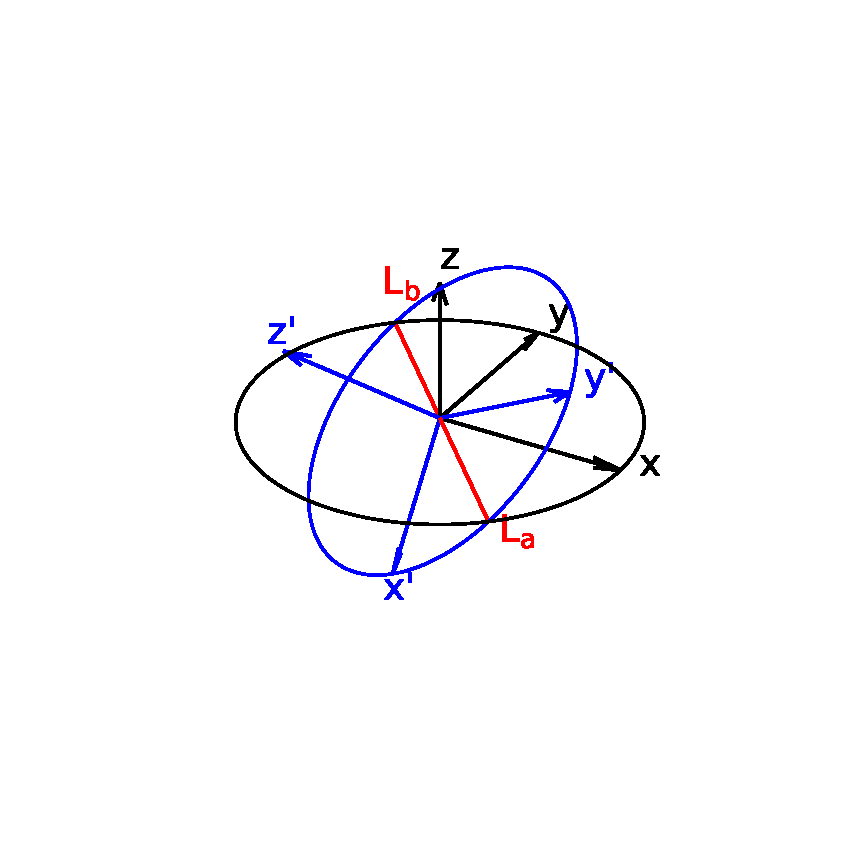
\includegraphics[width = 0.8\textwidth]{sections/TheoryGraphs/EulerAngle.eps}
	\vspace*{-2cm}
    \caption[Depiction of two Coordinate systems for description of Euler Angles.]{ Depiction of two coordinate systems  $\textbf{x},\textbf{y},\textbf{z}$ (black) and $\textbf{x}',\textbf{y}',\textbf{z}'$ (blue). 
			   The red cutting line of the $\textbf{xy}$ and $\textbf{x'y'}$ planes is between the vector $\textbf{L}_\mathrm{a}$ and $\textbf{L}_\mathrm{b}$.}
    \label{fig:EulerAngles}
\end{figure}

For the rotation of the CS it is necessary to apply the rotation matrices in a specific order.
The first rotation is around $\textbf{z}$ by the angle $\gamma$, followed by the rotation $\textbf{x}$ by $\beta$.
Then a rotation around the $\textbf{z}$ axis is done by the angle $\alpha$.
The rotation matrices $\textbf{R}_z(\theta)$, and $\textbf{R}_x(\theta)$ are mathematically described 
in Eq.~\eqref{eq:rotMatZ} and Eq.~\eqref{eq:rotMatX}, respectively.
These are the rotation matrices for a classical rotation around the $\textbf{z}$ and $\textbf{c}$ axes.
\begin{align}
	\label{eq:rotMatZ}
	\textbf{R}_z (\theta)  = \left(\begin{matrix}
					\cos(\theta) & -\sin(\theta) & 0 \\
					\sin(\theta) & \cos(\theta) & 0 \\
					0 & 0 & 1 \\
					\end{matrix} \right)
\end{align}

\begin{align}
	\label{eq:rotMatX}
	\textbf{R}_x (\theta)  = \left(\begin{matrix}
						1 & 0 & 0 \\
						0 & \cos(\theta) & -\sin(\theta)  \\
						0 & \sin(\theta) & \cos(\theta) \\
					\end{matrix} \right)
\end{align}

The full rotation of the coordinate system in dependency of the Euler angles is shown in Eq.~\eqref{eq:R_Euler}.

\begin{align}
	\label{eq:R_Euler}
	\textbf{R} = \textbf{R}_z (\gamma) \times \textbf{R}_x (\beta) \times \textbf{R}_z (\alpha)
\end{align}

\section{Electronic Structure Theory}
	In this report, properties derived from electronic structure theory are used for the training of the ML models.
	Although GFN2--xTB is used for this purpose, a short introduction to the Hartree--Fock model and Density Functional Theory is given.
	The introduction starts from the non--relativistic, stationary electronic Schrödinger--equation.
	From this the Hartree--Fock model will be derived.
	This is followed by Density Functional Theory, as this builds the theoretical basis of GFN2--xTB.
	After that the tight--binding method will be introduced from which the semiempirical method GFN2--xTB is derived.
	Atomic units are used for all equations in this section.

	\subsection{Hartree--Fock Model}
	Molecular systems in quantum mechanics can be described by a many--body wave function eigenvalue problem.
	The solution of this problem is given by solving the Schrödinger equation. The separation of its time--dependency, neglecting relativistic effects and
	the introduction of the \mbox{Born--Oppenheimer (BO) approximation} results in the electronic Schrödinger equation (Eq.~\eqref{eq:eSGl}).
	\begin{align}
		\label{eq:eSGl}
		\hat{H}_\mathrm{e} \Psi_\mathrm{e} = E_\mathrm{e} \Psi_\mathrm{e}
	\end{align}
 	The solution of this eigenvalue equation leads to the electronic energy $E_\mathrm{e}$.
	The electronic many--body--wave function $\Psi_\mathrm{e}$ of the system can be described by the Slater determinant (Eq.~\eqref{eq:SlaterD}).
	The use of the Slater determinant fulfills the condition of the antisymmetry of the wave function.
	The condition is due to the Pauli exclusion principle.
	The Slater determinant consists of $k$ spin--orbital wave functions $\phi_i$,
	and every wave function is permuted with the coordinates $\textbf{r}_i$ of the $N$ electrons.
	Furthermore, the wave function is normalized by the factor $(N!)^{-\frac{1}{2}}$.
	\begin{align}
		\label{eq:SlaterD}
		\Psi_\mathrm{e} = \dfrac{1}{\sqrt{N!}} \begin{vmatrix}
			\phi_1(\textbf{r}_1) & \phi_2(\textbf{r}_1)& \hdotsfor{1}&  \phi_k(\textbf{r}_1)\\
			\phi_1(\textbf{r}_2) &  \phi_2(\textbf{r}_2) & & \vdots\\
			\vdots& & \ddots& \vdots \\
			\phi_1(\textbf{r}_N)& \hdotsfor{1}& \hdotsfor{1} & \phi_k(\textbf{r}_N)\\
		\end{vmatrix}
	\end{align}
	The electronic Hamiltonian $\hat{H}_\mathrm{e}$ in the Hartree--Fock model is shown in Eq.~\eqref{eq:effHamiltonian}
	and consists of the kinetic energy of the electrons and the potential energy between electrons and nuclei as also between the electrons.
	Furthermore, the nuclear repulsion energy, which is approximated as a constant, is added.
	The kinetic energy of the nuclei can is separated, due to the \mbox{BO--approximation}.
	% Instead of the computation of every electron--electron interaction,
	% the electrons are assumed to be in an effective electronic potential,
	% which simplifies the hamiltonian to a sum of effective one--electron hamiltonians.
	% This is depicted in Eq.~\eqref{eq:effHamiltonian}.
	\begin{align}
		\label{eq:effHamiltonian}
		\hat{H}_\mathrm{e} = \sum_{A = 1}^{M} \sum_{i=1}^N \left( -\dfrac{1}{2}\nabla_i^2 - \dfrac{1}{|\textbf{R}_A - \textbf{r}_i|}\right) 
		+ \sum_{i=1}^N \sum_{\substack{j = 1 \\ i>j}}^N \dfrac{1}{|\textbf{r}_{i} - \textbf{r}_{j}|} 
		+ \sum_{A=1}^M \sum_{\substack{B=1\\ B>A}}^M \dfrac{Z_A Z_B}{|\textbf{R}_A - \textbf{R}_B|}
	\end{align}
	Here, $\textbf{R}_A$ is the coordinates of atom $A$, 
	$\textbf{r}_i$ the coordinates of electron $i$ and $Z_A$ the nuclear charge.
	While, $\nabla_i^2$ is the second derivative in respect to every coordinate of electron $i$.\\
	The electronic energy can now be described with the Slater determinant and Hamiltonian in Eq.~\eqref{eq:ElectronicEnergy}
	This leads to the description of the energy by the one--electron operator $h_i$,
	the coulomb operator $\hat{J}_i$ and the exchange operator $\hat{K}$.
	\begin{align}
		\label{eq:ElectronicEnergy}
		E_\mathrm{e} = \sum_{i=1}^N \braket{\phi_i | h_i | \phi_i} 
		+ \dfrac{1}{2} \sum_{i=1}^N \sum_{j=1}^N \left(\braket{\phi_j | \hat{J}_i | \phi_j} 
		- \braket{\phi_j | \hat{K}_i | \phi_j}\right)
	\end{align}

	The Rayleigh--Ritz variational principle (s. Eq.~\eqref{eq:RayleighRitzVP}) states,
	that the total energy $E_0$ of the system is always beneath or equal
	to the energy corresponding to the approximated wave function.
	This allows the search of the exact energy by optimizing the wave function (or its parameters).
	\begin{align}
		\label{eq:RayleighRitzVP}
		E_0 \leq \braket{\Psi | \hat{H} | \Psi}
	\end{align}
	Hence, the determination of the total energy of the system is an eigenvalue problem and can be solved by minimization.
	To minimize the energy, Lagrangian optimization is employed, under the condition of orthonormal $\phi_i$.
	The inner product of the wave function $\braket{\phi_i|\phi_j} = \delta_{ij}$ corresponds to the Kronecker delta. 
	The Kronecker delta is $\delta_{ij} = 0$ if $i$ and $j$ are not equal, and $\delta_{ij} = 1$ if $i$ and $j$ are equal.
	The derivative of the Lagrangian functional leads to the canonical Fock equation \eqref{eq:FockEquation},
	which is a solution for the minimal energy.

	\begin{align}
		\hat{f}(\textbf{r}_i) \phi_k(\textbf{r}_i) &= \epsilon(\textbf{r}_i) \phi_k(\textbf{r}_i)
		\label{eq:FockEquation}\\
		\hat{f}(\textbf{r}_i) &= \hat{h} + \sum_{j=1}^N (2 \hat{J}_j - \hat{K}_j)
	\end{align}

	The Fock--operator $\hat{f}(\textbf{r}_i)$ is an effective one--electron operator.
	This enables the determination of the spin--orbital wave functions in an iterative manner,
	as the Fock--operator itself depends on the spin--orbital wave functions.
	The iterative search is possible due to the self--consistency of the Hartree--Fock equation.
	Furthermore, the general optimization can be achieved due to the Rayleigh--Ritz variational principle.
	Important to point out is that the Fock--operator consists of the one--electron operator, the exchange--operator
	and the coulomb operator, while the correlation is not included. \\
	The spin--orbital wave functions are described via a basis set approximation.
	This LCAO--approach is shown in Eq.~\eqref{eq:BasisSet},
	where the spin--orbital wave--functions are the sum of $K$ basis functions with an associated constant.
	\begin{align}
		\label{eq:BasisSet}
		\phi_i(\textbf{r}) = \sum_\mu^K c_\mu \chi_\mu (\textbf{r})
	\end{align}
	Merging the basis--set approach into Eq.~\eqref{eq:FockEquation} leads to Roothaan--Hall equation shown in Eq.~\eqref{eq:FCSCe}.
	Here, $\textbf{F}$ is the Fock matrix, $\textbf{C}$ a matrix of coefficients $c_\mu$,
	$\textbf{S}$ the overlap matrix and $\bm{\upepsilon}$ the diagonal eigenvalue matrix.
	This equation is used find a solution for the energy iteratively.
	Starting with an initial guess of the Fock matrix,
	the matrix $\textbf{C}$ is computed, with this matrix, the density matrix $\textbf{D}$ is calculated. 
	From the matrix $\textbf{D}$, is then used for the calculation of the new Fock matrix.
	\begin{align}
		\label{eq:FCSCe}
		\textbf{F} \textbf{C} = \textbf{S} \textbf{C} \bm{\upepsilon}
	\end{align}
	% \textcolor{blue}{There is an infinite large number of possible solutions for the spin--orbital wave functions,
	% which leads to high computational cost and capacity for solving.
	% For the simplification, a basis set of a LCAO--approach is used for the computation of the spin--orbital wave function.}
	% \begin{align}
	% 	\phi(\textbf{r}) = \sum_\mu^K c_\mu \chi_\mu(\textbf{r})
	% \end{align}
	% \subsection{Kohn--Sham Density Functional Theory}
	% The molecule--orbital wave functions $\psi_i$ is approximated with basis sets, shown in Eq.~\eqref{eq:BasisSet}
	% \begin{align}
	% 	\label{eq:BasisSet}
	% 	\psi_i = \sum^{A}_{i} \chi 
	% \end{align}
	\subsection{Kohn--Sham Density Functional Theory}
	As mentioned above, the correlation between electrons is not described in the Hartree--Fock model,
	due to the use of a single Slater determinant.\\
	The correlation energy can be described by two different approaches.
	Instead of using one single Slater determinant, a linear combination of Slater determinants can be used.
	This leads to the post--Hartree--Fock methods like Full--CI or MP2.
	The second approach is the Density Functional Theory (DFT).\\
	The Hohenberg--Kohn theorems build the basis for the DFT.
	These two theorems postulate, that the energy is a functional of the density,
	and that this functional follows the variational principle.\\
	The description of the energy can therefore be done via the density of the electrons,
	which is defined in Eq.~\eqref{eq:Density}.
	Where, $n_\mathrm{occ}$ is the occupation number of the spin--orbital wave function.
	\begin{align}
		\label{eq:Density}
		\rho(\textbf{r}) = n_\mathrm{occ} \sum_{i=1}^n  |\phi_i(\textbf{r})|^2
	\end{align}
	The general approach is to describe the energy in dependence of the electron density $E[\rho]$.
	There are different approaches for this connection. 
	The most known approach, Kohn--Sham Density Functional Theory (KS--DFT), will be discussed.
	The energy in KS--DFT consists of the inexact kinetic energy, coulomb integral,
	the exchange correlation energy and the potential field.
	The kinetic energy is inexact, due to the assumption of non--interacting electrons.
	The energy $E_\mathrm{XC}$ consists mainly of the correlation energy and the exchange energy.
	In theory, the energy $E_\mathrm{XC}$ should also include the self interaction energy and a correction to the kinetic energy.
	\begin{align}
		\label{eq:EnergyDFT}
		E[\{\phi_i\}] = T[\{\phi_i\}] + J[\rho] + E_\mathrm{XC}[\rho] + \int v(\textbf{r}) \rho(\textbf{r}) \mathrm{d}\textbf{r}
	\end{align}
	The minimization of the energy is done by a Lagrangian optimization with analogue conditions compared to Hartree--Fock.
	This leads to the Kohn--Sham operator and a new eigenequation, which is shown in Eq~\eqref{eq:KSEigeneq}.
	\begin{align}
		\hat{f}^\mathrm{KS}(\textbf{r}_i) \phi_k(\textbf{r}_i) &= \epsilon(\textbf{r}_i) \phi_k(\textbf{r}_i)\label{eq:KSEigeneq}\\
		\hat{f}^\mathrm{KS}(\textbf{r}_i) &= \hat{h}_i + 2 \sum^n_{j=1} \hat{J}_j + \hat{v}_\mathrm{xc} 
	\end{align}
	In comparison to the Fock operator, $\hat{f}^\mathrm{KS}(\textbf{r}_i)$ includes an exchange--correlation term, instead of the exchange operator.
	With a basis set approach analogue to the HF model,
	an eigenvalue equation similar to the Roothaan--Hall equation is derived.
	% The spin--orbital wave functions are described via a basis set approximation.
	% This LCAO--approach is shown in Eq.~\eqref{eq:BasisSet},
	% where the spin--orbital wave--functions are the sum of $K$ basis functions with an associated constant.
	% \begin{align}
	% 	\label{eq:BasisSet}
	% 	\phi_i(\textbf{r}) = \sum_\mu^K c_\mu \chi_\mu (\textbf{r})
	% \end{align}
	% Merging the basis--set approach into the Kohn--Sham eigenequation leads to a matrix eigenequation shown in Eq.~\eqref{eq:FCSCe}.
	% Here, $\textbf{F}$ is the Fock matrix, $\textbf{C}$ a matrix of coefficients,
	% $\textbf{S}$ the overlap matrix and $\bm{\upepsilon}$ the diagonal eigenvalue matrix.
	% This equation can now be used to find a solution for the energy iteratively.
	% Starting with an initial guess of the Fock matrix,
	% the matrix $\textbf{C}$ is computed, with this matrix, the density matrix $\textbf{D}$ is calculated. 
	% From the matrix $\textbf{D}$, is then used for the calculation of the new Fock matrix.
	\begin{align}
		\label{eq:FCSCe}
		\textbf{F} \textbf{C} = \textbf{S} \textbf{C} \bm{\upepsilon}
	\end{align}

	% -Variatonelles system beibehlaten --> dichte funktional theorie hat korellationsenergie
	% -verwendet dichte --> zweites Hohenberg--Kohn theorem zegit, dass es auch das variatonell ist 
	% -energie ist also funktional der dichte
	% -operator einführen
	% -FC = SCe enführen zum schluss --> lösung beschreiben
	% -WF die verwendet werden --> erst bei GFN2--xTB
	% -Basissatznäherung auch mit rein 

	\subsection{GFN2--xTB Electronic Structure Method}
	GFN2--xTB is a Density Functional Tight Binding (DFTB) method,
	that is optimized for \textbf{G}eomteries,
	\textbf{F}requencies and \textbf{N}oncovalent interaction energies.
	In these DFTB methods, the electron density $\rho_0$ is a linear combination of atomic electron densities $\rho_{0,A}$.
	\begin{align}
		\label{eq:GFN2:Rho0}
		\rho_0 = \sum_A \rho_{0,A}
	\end{align}
	The energy is following expanded by a Taylor series around the electron density $\rho_0$.
	In GFN2--xTB the expansion is done up to the third order.
	\begin{align}
		\label{eq:GFN2:EnergyPerturbation}
		E[\rho] = E^{(0)}[\rho_0] + E^{(1)}[\rho_0,(\delta \rho)]
		 + E^{(2)}[\rho_0,(\delta \rho)^2]+ E^{(3)}[\rho_0,(\delta \rho)^3] + \dots
	\end{align}
	Furthermore, the energy is described with the kinetic energy $T[\rho(\textbf{r})]$ and
	the external potential, due to the nuclei $V_n(\textbf{r})$.
	A local density approximation (LDA) is used for the description of the exchange--correlation energy $\epsilon^\mathrm{LDA}_\mathrm{XC}$.
	As the LDA neglects the long range correlation effects,
	these are described via a non--local correlation contribution $\Phi^\mathrm{NL}_\mathrm{C}\left(\textbf{r},\textbf{r}^\prime\right)$.
	This is in contrast to other DFTB methods like DTFB3.
	\begin{align}
		\label{eq:GFN2:EnergyDFT}
		\begin{split}
		E[\rho] &= \int \rho(\textbf{r})\bigg[ T[\rho(\textbf{r})]
		 + V_n(\textbf{r}) 
		 + \epsilon^\mathrm{LDA}_\mathrm{XC}[\rho(\textbf{r})] \\
		 &+ \dfrac{1}{2} \int \left( \dfrac{1}{|\textbf{r}-\textbf{r}^\prime|} 
		 + \Phi^\mathrm{NL}_\mathrm{C}\left(\textbf{r},\textbf{r}^\prime\right)\right)
		 \rho\left(\textbf{r}^\prime\right)\mathrm{d}\textbf{r}^\prime \bigg] \mathrm{d}\textbf{r} + E_{nn}
		\end{split}
	\end{align}
	The terms of Eq.~\eqref{eq:GFN2:EnergyPerturbation} can be divided into different energy contributions.
	These contributions will be briefly discussed.
	The zeroth order term shown in Eq.~\eqref{eq:GFN2:E_0} consists of the repulsion energy~$E_\mathrm{rep}^{(0)}$ and
	dispersion energy~$E_\mathrm{disp}^{(0)}$. These are typically described by Buckingham or Lennard--Jones potentials.
	The dispersion term arises, due to the non--local correlation functional.
    Furthermore, the zeroth order term energy of the valence electrons $E_\mathrm{A,valence}^{(0)}$
	and core electron $E_\mathrm{A,core}^{(0)}$ is summed, though the energy of the core electrons is defined as zero.

    \begin{align}
        \label{eq:GFN2:E_0}
        E[\rho_0] \approx E_\mathrm{rep}^{(0)} + E_\mathrm{disp}^{(0)} + \sum_A \left(E_\mathrm{A,valence}^{(0)} + E_\mathrm{A,core}^{(0)}\right)
    \end{align}	

	The first order perturbation energy $E^{(1)}[\rho_0,(\delta \rho)]$
	is approximately described by a first order dispersion energy $E_\mathrm{disp}^{(1)}$,
	and first order valence electron energy $E_\mathrm{A,valence}^{(1)}$.
	This perturbation allows the description of covalent bonding,
	as the electron density so far is described as spherical densities around the atoms, with no interaction.
	\begin{align}
        \label{eq:GFN2:E_1}
		E^{(1)}[\rho_0,(\delta \rho)] \approx E_\mathrm{disp}^{(1)} + \sum_A E_\mathrm{A,valence}^{(1)}
    \end{align}

The second order energy perturbation $E^{(2)}[\rho_0,(\delta \rho)^2]$ is described by the contribution of dispersion,
electrostatics and exchange correlation energies.
The exchange and correlation energy~$E_\mathrm{XC}^{(2)}$
and electrostatic energy~$E_\mathrm{ES}^{(2)}$ are described in GFN2--xTB with an isotropic as also an anisotropic contribution.
This is in contrast to other DFTB methods, where only a monopole approximation is done.
Hence, there is only an isotropic description in other methods.
	\begin{align}
        \label{eq:GFN2:E_2}
		E^{(2)}[\rho_0,(\delta \rho)^2] \approx E_\mathrm{ES}^{(2)} + E_\mathrm{XC}^{(2)} + E_\mathrm{disp}^{(2)}
    \end{align}	
	For the third order perturbation, 
	only the electrostatic and exchange correlation energies are used and computed with the Mulliken approximation.
	All other contributions to the third order perturbation are neglected.
	\begin{align}
        \label{eq:GFN2:E_3}
		E^{(3)}[\rho_0,(\delta \rho)^3] \approx  E_\mathrm{ES}^{(3)} + E_\mathrm{XC}^{(3)} 
    \end{align}	
Merging all energy contributions shown in Eq.~\eqref{eq:GFN2:E_0} to Eq.~\eqref{eq:GFN2:E_3} into Eq.~\eqref{eq:GFN2:EnergyPerturbation} leads to Eq.~\eqref{eq:GFN2:E}.
Though, some further adjustments are done. The isotropic contribution of the electrostatic and exchange correlation energies are described by a single term $E_\mathrm{IES+IEC}$.
While the anisotropic electrostatic energy~$E_\mathrm{AES}$ and anisotropic exchange correlation energy~$E_\mathrm{AXC}$ are described separately.
The valence electron energy contributions are described via the extended Hückel type energy~$E_\mathrm{EHT}$.
Independent of the above discussed perturbation, an energy term~$G_\mathrm{Fermi}$ describing the Fermi--smearing  is included,
which leads to the complete energy equation shown in Eq.~\eqref{eq:GFN2:E}.
	\begin{align}
		\label{eq:GFN2:E}
		E_\mathrm{GFN2-xTB} =  E_\mathrm{rep} + E_\mathrm{EHT} + E_\mathrm{disp} 
		+ E_\mathrm{IES+IEC} + E_\mathrm{AES} + E_\mathrm{AXC} + G_\mathrm{Fermi}
	\end{align}
	The wave function is approximated by a minimal valence basis set STO--$m$G.
	The energy is computed similar to KS--DFT and Hartree Fock.
	The Roothaan--Hall type Eq.~\eqref{eq:FCSCe} is solved in a selfconsistent manner.


    \section{Hessian Matrices}
	Hessian matrices are required for several uses like the computation of wave numbers or thermodynamic quantities.
	Furthermore, they are necessary for the transition state search.
	The hessian matrix is a $3M \times 3M$ matrix of second derivatives
	of the energy in respect to every permuted atom coordinate pair in the system.
	\begin{align}
		\textbf{H} =
		\left(\begin{matrix}
			\dfrac{\partial^2 E}{\partial x_A \partial x_A} & \hdotsfor{1} & \dfrac{\partial^2 E}{\partial x_A \partial y_M} &
			\dfrac{\partial^2 E}{\partial x_A \partial z_M} \\	
			\dfrac{\partial^2 E}{\partial x_A \partial y_A} & \ddots & & \vdots \\
			\vdots & & \ddots & \vdots \\
			\dfrac{\partial^2 E}{\partial z_N \partial x_A}  & \hdotsfor{0} & & \dfrac{\partial^2 E}{\partial z_M \partial z_M} 
		\end{matrix}\right)
	\end{align}
	The hessian matrix can be divided into $M^2$ $3 \times 3$ block matrices,
	where each depends on the coordinates of an atom pair.
	Theses $3 \times 3$ block matrices are beneficial for the prediction, as they only depend on two atoms.
	Hence, only information about the two atoms need to be given to the machine learning model to predict the block matrix.
	\begin{align}
		\textbf{H} =
		\left(\begin{matrix}
			\textbf{H}^{AA} & \textbf{H}^{AB} & \hdotsfor{0} &  \textbf{H}^{AM}\\
			\textbf{H}^{BA}& \ddots & & \vdots\\
			\vdots & & \ddots & \vdots \\
			\textbf{H}^{MA} &\hdotsfor{0} & \hdotsfor{0}& \textbf{H}^{MM} \\
		\end{matrix}\right)
	\end{align}
	Due to the Schwartz Theorem, the $\textbf{H}^{BA}$ and $\textbf{H}^{AB}$ are related to another by Eq.~\eqref{eq:Hess:HABBA}
	\begin{align}
		\label{eq:Hess:HABBA}
		\textbf{H}^{BA} = \left({\textbf{H}^{AB}}\right)^\intercal
	\end{align}
	Therefore the only information needed for the hessian is a triangular matrix (s.~Eq.~\eqref{eq:Hess:TriangularMat}).
	\begin{align}
		\label{eq:Hess:TriangularMat}
		\textbf{H} =
		\left(\begin{matrix}
			\textbf{H}^{AA} & \textbf{H}^{AB} & \hdotsfor{0} &  \textbf{H}^{AM}\\	
			 & \ddots & & \vdots \\
			 & \text{\kern-2em\smash{\raisebox{-2ex}{\Huge 0}}} & \ddots & \vdots \\
			 &  &  & \textbf{H}^{MM} 
		\end{matrix}\right)
	\end{align}

	--Projection of the Hessian matrix\\

	--Mass weighting the projected hessian matrix.\\

	--Test this \\

	\section{Machine Learning}
	Extra Tree Regression (ETR) and Random Forest Regression (RFR) are used as ML algorithms in this research.
	Both algorithms are ensemble methods based on decision trees as individual estimators.
	In this section, decision tree based algorithms will be discussed,
	and the differences between the ETR and RFR will be emphasized.\\
	Often these decision tree based algorithms are based on the Classification and Regression Tree (CART) algorithm.
	For an example, a response $Y$ that depends on two variables $X1$ and $X2$ is assumed.
	The variables $X1$ and $X2$ are called features.
	A tree based model splits the space of this function into several recursive binary partitions.
	Recursive binary means in this case, that the splits are orthogonal to the axis of the features.
	This split is shown on the left in Fig.~\ref{fig:ML_Split}.
	\begin{figure}[H]
		\centering
		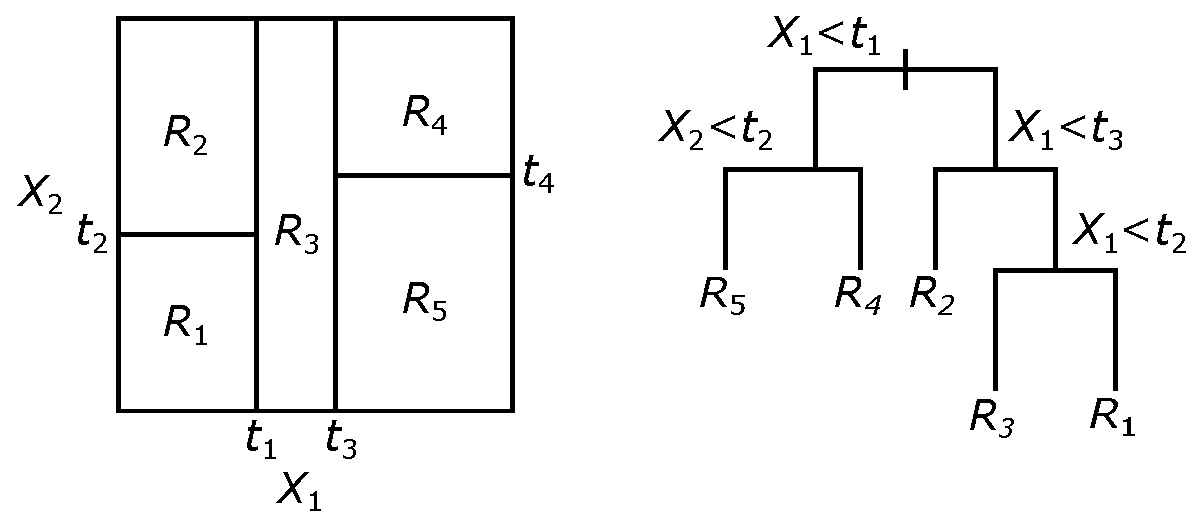
\includegraphics[width = \textwidth]{sections/TheoryGraphs/ZeichnungDecisionTree_Rectangle.eps}
		\caption[Structure of a CART split and its resulting Decision Tree]{
		The recursively binary grown split is shown on the left. On the right, the resulting Decision Tree is depicted.}
		\label{fig:ML_Split}
	\end{figure}
	In each partition $Y$ is modeled with a function or constant $R_i$.
	The splitting points $t_1$ to $t_4$ are chosen differently for the RFR and ETR.
	In RFR, the splitting point is determined by choosing the best feature and of this feature the best split value.
	Hence, it is a two dimensional search.
	In the case of the ETR, the feature is chosen randomly.
	After that, the best split value for this feature is chosen.
	The relation between the features and the partitioned response $Y$ can be depicted in a decision tree,
	which is shown in Fig.~\ref{fig:ML_Split} on the right.
	This can also be described mathematically via Eq.~\eqref{eq:DTfunc}
	\begin{align}
		\label{eq:DTfunc}
		\hat{f}(X) = \sum_{m=1}^5 c_m I\{(X_1,X_2) \in R_m \}
	\end{align}
	Here, $\hat{f}(X)$ is the function that describes the response $Y$.
	Each region $m$ has a corresponding constant $c_m$. The function $I$ can either be $I=1$,
	if the features $X_1$ and $X_2$ are in the rectangle $R_m$, or it is $I=0$, if it is not the case.
	Originally, the ETR and RFR have another difference, which is that the ETR did not use bootstrapping.
	Bootstrapping uses the training set and makes several new training sets from this.
	The new training sets are randomly filled with the datasets of the original training set.


	
	
\section{Feature Overview}
	In this section an overview of the used features is given.
	The quantities used for the feature vector are depicted in Tab.~\ref{tab:Feature}
	and are generated with the GFN2--xTB method. The features are mostly atom centered quantities
	and are based on geometry, density or energy.
	The features were calculated for the systems in the APF CS.\\
	There are quantities, which also have an extended version.
	If this is the case, a tick is set at Extension.
	The quadrupole moment matrix $\bm{\Uptheta}$ was reduced to a vector by the multiplication
	with a one vector $\underline{1}$ (s.~Eq~\eqref{eq:redTheta}).
	\begin{align}
		\label{eq:redTheta}
		\bm{\uptheta} = \bm{\Uptheta} \times \underline{1}
	\end{align}

	\begin{table}[H]
		\centering
		\caption{List of quantities used for the ML models as features.
				The quantities are divided into geometry,
				density and energy based quantities.}
			\begin{tabular}{l l l}
				\hline
				Feature &  Description& Extension\\
				\hline
				\textbf{Geometry} & & \\
				$CN$ & Coordination Number & \checkmark \\
				\hline

				\textbf{Density} && \\
				$\bm{\upmu}$ & Dipole Moment & \checkmark \\
				$\bm{\upmu}_\mathrm{Z}$ & Dipole Moment, only Z direction & \\
				$\bm{\uptheta}$ & Quadrupole Moment & \checkmark\\
				\hline

				\textbf{Energy} && \\
				$E_\mathrm{resp}$ & Response& \\
				$E_\mathrm{gap}$ & HOMO -- LUMO gap& \checkmark\\

				$\mu_\mathrm{pot}$& Chemical Potential & \checkmark\\

				$\epsilon_\mathrm{HOAO}$ & Atomic HOMO & \checkmark \\

				$\epsilon_\mathrm{LUAO}$ & Atomic LUMO & \checkmark \\

				$E_\mathrm{rep}$ & Repulsion & \\
				$E_\mathrm{EHT}$ & extended Hückel theory& \\
				$E_\mathrm{disp}^{(2)}$ & Dispersion 2$^\mathrm{nd}$ order & \\
				$E_\mathrm{disp}^{(3)}$ & Dispersion 3$^\mathrm{rd}$ order & \\
				$E_\mathrm{IES+IXC}$ & Isotropic ES and XC & \\
				$E_\mathrm{AES}$ & Anisotropic ES& \\
				$E_\mathrm{AXC}$ & Anisotropic XC & \\
				$E_\mathrm{tot}$ & Total Energy & \\
				\hline 
			\end{tabular}
		\label{tab:Feature}
	\end{table}
	Each quantity is atom specific, thus each quantity is there from atom $A$ and $B$.
	The quantities shown in Tab.~\ref{tab:Feature} are all further processed for the use as features.
	From the quantities $x_A$ and $x_B$ the arithmetic mean,
	the product and absolute difference is calculated (s. Eq.~\eqref{eq:FeatureProcess}).
	The new quantities $X_\mathrm{Arith}$,
	$X_\mathrm{Prod}$ and $X_\mathrm{AbsDiff}$ are used as the features for the ML model.
	\begin{subequations}
		\label{eq:FeatureProcess}
		\begin{align}
			X_\mathrm{Arith}&= \dfrac{x_A + x_B}{2}\\
			X_\mathrm{Prod}&= x_A \cdot x_B \\
			X_\mathrm{AbsDiff}&= | x_A - x_B | 
		\end{align}
	\end{subequations}
	So far the feature $X$ is build up by $X = \{X_\mathrm{Arith},X_\mathrm{Prod},X_\mathrm{AbsDiff}\}$.
	If such feature is connected to the hessian matrices,
	it is independent for every element in a hessian matrix block $\textbf{H}_{AB}$.
	Hence, the ML model is not able to distinguish the elements.
	Two ways were developed and tested, which distinguish the elements.
	At first, the feature is increased by indices specific for each element. The indices are shown in Tab.~\ref{tab:Indices}
	\begin{table}[H]
		\centering
		\caption{Indices used for the different elements in a hessian matrix block to differ between the elements.}
			\begin{tabular}{c c c c | c }
				\hline
				& &  Indexed& & Permuted \\
				Hessian element &  $x^\mathrm{idx}$ & $y^\mathrm{idx}$ & $z^\mathrm{idx}$ & Index\\
				\hline
				\\[-1em]
				$\dfrac{\partial^2 E}{\partial x_A \partial x_A}$ & 2 & 0 & 0 & 0\\
				\\[-1em]
				$\dfrac{\partial^2 E}{\partial x_A \partial y_A}$ & 1 & -1 &  0 & 1\\
				\\[-1em] 
				$\dfrac{\partial^2 E}{\partial x_A \partial z_A}$ & 1 & 0 &  -1 & 2\\
				\\[-1em]
				$\dfrac{\partial^2 E}{\partial y_A \partial x_A}$ & -1 & 1 &  0 & 1\\
				\\[-1em]
				$\dfrac{\partial^2 E}{\partial y_A \partial y_A}$ & 0 & 2 &  0 & 0\\
				\\[-1em]
				$\dfrac{\partial^2 E}{\partial y_A \partial z_A}$ & 0 & 1 &  -1 & 2\\
				\\[-1em]
				$\dfrac{\partial^2 E}{\partial z_A \partial x_A}$ & -1 & 0 &  1 & 2\\
				\\[-1em]
				$\dfrac{\partial^2 E}{\partial z_A \partial y_A}$ & 0 & -1 &  1 & 2\\
				\\[-1em]
				$\dfrac{\partial^2 E}{\partial z_A \partial z_A}$ & 0 & 0 &  2 & 3\\
				\\[-1em]
				\hline 
			\end{tabular}
		\label{tab:Indices}
	\end{table}

	The feature vector is expanded with these indices
	$ X  = \{x^\mathrm{idx},y^\mathrm{idx},z^\mathrm{idx},X_\mathrm{Arith},X_\mathrm{Prod},X_\mathrm{AbsDiff}\}$.
	This labeling is called \textbf{indexed} (idx).\\
	In another approach, the hessian matrix is further rotated,
	so that the hessian elements are on the same spot for every prediction.
	In the same way, the feature quantities are adapted. The adapted matrix and coordinate system are shown in the Appendix 

	
	\begin{table}[H]
		\centering
		\caption[]{Permutation of the coordinates for each Hessian element.}
			\begin{tabular}{c c c c c}
				\hline
				Hessian Element & x & y & z \\
				\hline \\[-1em]
				$\dfrac{\partial^2 E}{\partial x_A \partial x_A}$ & x & y & z & \\ [+0.7em]
				$\dfrac{\partial^2 E}{\partial x_A \partial y_A}$ & y & x & $-$z & \\[+0.7em]
				$\dfrac{\partial^2 E}{\partial x_A \partial z_A}$ & z & x & y & \\[+0.7em]

				$\dfrac{\partial^2 E}{\partial y_A \partial x_A}$ & x & y & z & \\[+0.7em]
				$\dfrac{\partial^2 E}{\partial y_A \partial y_A}$ & y & z & x & \\[+0.7em]
				$\dfrac{\partial^2 E}{\partial y_A \partial z_A}$ & z & y & $-$x & \\[+0.7em]

				$\dfrac{\partial^2 E}{\partial z_A \partial x_A}$ & x & z & $-$y & \\[+0.7em]
				$\dfrac{\partial^2 E}{\partial z_A \partial y_A}$ & y & z & x & \\[+0.7em]
				$\dfrac{\partial^2 E}{\partial z_A \partial z_A}$ & z & x & y & \\[+0.7em]
				\hline

			\end{tabular}
		\label{tab:Permutation}
	\end{table}



	After that, an index is put onto the features again. 
	In this case though, the hessian matrix elements with a derivative in respect to the $z$ coordinate get the same index.
	Furthermore, the diagonal and off--diagonal elements get different indices.
	This labeling is called \textbf{permuted} (perm).
	%CCCCCCCCCCCCCCCCCCCCCCCCCCCCCCCCCCCCCCCCCCCCCCCCCCCCCCCCCCCCCCCCCCCCCCCCCCCCCCCCCCCCCCCCCCCCC
	\section{Transformation of Coordinates}
	The hessian matrix and some features depend on the orientation of the coordinate~system~(CS).
	For the ML model a consistent orientation for every atom pair is necessary.
	Furthermore, the hessian elements shall be learned atom pair wise.
	Thus, the orientation of the molecule is brought into atom pair focused CS,
	where the origin of the CS is in the center of the considered atom pair,
	while both atoms are on the z--Axis.
	In this section,
	the transformation of the initial coordinate system into the atom pair focused CS will be discussed.\\
	The initial CS is not fixed to any constraints.
	Therefore, the initial CS is transformed into the main inertia system,
	from which the transformation to the atom pair focused coordinate systems is performed.\\
	At first a translation of the origin of the initial CS to the center of mass is done by Eq.~\eqref{eq:TransIinitCenterMass}.
	
	\begin{align}
		\textbf{r}^\mathrm{s}_A =  \textbf{r}^\mathrm{init}_A - \textbf{s}^\mathrm{init}
		\label{eq:TransIinitCenterMass}
	\end{align}
	Where $\textbf{r}^\mathrm{s}_A$ is the coordinate vector of an atom $A$ in the mass centered CS, $\textbf{r}^\mathrm{init}_A$ the coordinate vector in the initial CS and $\textbf{s}^\mathrm{init}_A$ is the center of mass in the initial CS, and is defined in Eq.~\eqref{eq:CenterOfMass}.
	
	\begin{align}
		\textbf{s}^\mathrm{init} = \dfrac{1}{M} \sum_{A}^{N} m_A \cdot \textbf{r}^\mathrm{init}_A
		\label{eq:CenterOfMass}
	\end{align}
	Here $m_A$ is the mass of atom $A$, $M$ is the mass of the molecule and $N$ the number of atoms in the molecule.
	Once the origin of the new CS is determined,
	the orientation of its axes is arranged to the moment of inertia as computed by Eq.~\eqref{eq:MomentOfInertia}.
	
	\begin{align}
		\textbf{I}^\mathrm{s} = \left(\begin{matrix}
						I_{xx} & I_{xy} & I_{xz} \\
						I_{yx} & I_{yy} & I_{yz} \\
						I_{zx} & I_{zy} & I_{zz} \\ 
				   	\end{matrix} \right) 
			 ; I_{ab} = \begin{cases}
				\sum_{A}^{N} m_A ( b_A^2 + c_A^2 ) ~~\mathrm{if}~ a = b\\
			   	 - \sum_{A}^{N} m_A \cdot a_A \cdot b_A  ~\mathrm{if}~ a \neq b \\
			   	\end{cases} a,b \in x,y,z
		\label{eq:MomentOfInertia}
	\end{align}
	
	For the computation of the elements $I_{ab}$ of the inertia tensor $\textbf{I}^\mathrm{s}$ the diagonal
	elements and non--diagonal elements are divided in two cases.
	Here, $a$ and $b$ are variables for the spatial directions of the coordinates~$x,y$ and $z$.
	For the rotation of the mass centered origin CS into the main inertia system,
	the matrix $\textbf{R}_\mathrm{mi}^\mathrm{init}$ of eigenvectors of the inertia tensor $\textbf{I}^\mathrm{s}$ is needed.
	For that, the eigenvectors $\textbf{R}_\mathrm{mi}^\mathrm{init}$ are computed
	by solving the eigenvalue equation.
	The eigenvalues are then used to get the eigenvectors.
	To assure, that the matrix $\textbf{R}_\mathrm{mi}^\mathrm{init}$ is a right--handed matrix the determinant is calculated.
	If the determinant is negative, the sign of the third eigenvector is changed. Furthermore, it needs to be assured,
	that the eigenvector is consistently rotated in the same direction, independent of the outgoing position.
	The chosen constraint is, that the highest value of the eigenvectors are positive,
	if this is not the case the sign of the eigenvector and the next eigenvector in $\textbf{R}_\mathrm{mi}^\mathrm{init}$ is changed.\\
	The rotation of the coordinates is done by Eq.~\eqref{eq:rotCoord}.
	\begin{align}
		\textbf{r}_A^\mathrm{mi} = \textbf{R}_\mathrm{mi}^\mathrm{init} \textbf{r}_A^\mathrm{s}
		\label{eq:rotCoord}
	\end{align}
	Here, $\textbf{r}_A^\mathrm{mi}$ is the coordinate of an atom $A$ in the main inertia CS.
	The rotation is done for every atom in the molecule. After that operation,
	the molecule is in the main inertia CS.\\ The hessian matrix also depends
	on the CS and therefore needs to be rotated, too.
	A translation is not needed. Eq.~\eqref{eq:rotHessian} describes
	the rotation of the hessian matrix in the initial CS to the main inertia system.
	For this a $3N \times 3N$ rotation matrix $\textbf{P}_\mathrm{mi}^\mathrm{init}$ needs to be constructed,
	where the diagonal 3 x 3 blocks are $\textbf{R}_\mathrm{mi}^\mathrm{init}$.
	This matrix is shown in Eq.~\eqref{eq:rotMatrixHessian}.
	\begin{align}
		\label{eq:rotMatrixHessian}
		\textbf{P}_\mathrm{mi}^\mathrm{init} = \left(\begin{matrix}
							\textbf{R}_\mathrm{mi}^\mathrm{init} &\text{\Large\textbf{0}}& && \text{\Large\textbf{0}}  \\
							\text{\Large\textbf{0}}& \textbf{R}_\mathrm{mi}^\mathrm{init} & & &\text{\Large\textbf{0}} \\
							\text{\Large\textbf{0}} & & \ddot& &\\
							 & & &\ddot & \text{\Large\textbf{0}}\\
							\text{\Large\textbf{0}}& & & \text{\Large\textbf{0}} &\textbf{R}_\mathrm{mi}^\mathrm{init}
							\end{matrix}\right)
	\end{align}

	\begin{align}
		\textbf{H}^\mathrm{mi} =\textbf{P}_\mathrm{mi}^\mathrm{init} \times \textbf{H}^\mathrm{init} \times {\left(\textbf{P}_\mathrm{mi}^\mathrm{init}\right)}^\intercal
		\label{eq:rotHessian}
	\end{align}
	The hessian matrix in the initial system is $\textbf{H}^\mathrm{init}$,
	while the hessian matrix in the main inertia system is $\textbf{H}^\mathrm{mi}$.\\
	In the following, the transformation of the main inertia CS to the atom pair focused CS will be discussed.
	The transformation starts with the translation of the origin to the center of an atom pair.
	The translation is described with Eq.~\eqref{eq:TranslationInertiaAPF}.\\
	\begin{align}
		\textbf{r}^\mathrm{mi,c}_C = \textbf{r}^\mathrm{mi}_C -
		 \left(\dfrac{1}{2} \textbf{r}^\mathrm{mi}_A + 
		 \dfrac{1}{2}\textbf{r}^\mathrm{mi}_B \right) 
		 \mathrm{for}~A,B,C \in A, B, ..., N
		\label{eq:TranslationInertiaAPF}
	\end{align}
	After this operation, the origin of the CS is in the center of the atom pair.
	To fix the orientation, the atom pair is aligned along the z--axis.
	The Euler angles are used to determine the rotation matrix.
	The rotation of the CS depends on the considered atom pair.
	It is divided into whether $A = B$ or $A \neq B$.
	At first the construction of the rotation matrix for the case $A \neq B$ will be discussed.\\
	The z--axis of the atom pair focused CS is aligned to $\textbf{r}^\mathrm{mi,c}_A$.
	The x--axis is defined in Eq.~\eqref{eq:x_axis}, where $\textbf{z}$ is a unit vector in z--direction of the atom pair focused CS,
	and $\bm{\upmu}_A$ is the dipole moment of the atom $A$.
	\begin{align}
		\textbf{x} = \textbf{z} \times ( \mathrm{\bm{\upmu}_{A}} + \mathrm{\bm{\upmu}_{B}})
		\label{eq:x_axis}
	\end{align}
	The cutting line $\textbf{L}$ of the xy--plane of the atom pair focused CS and xy--plane of the centered main inertia CS
	is described with Eq.~\eqref{eq:EulerLL}.
	\begin{align}
		\label{eq:EulerLL}
		\mathbf{L} = \mathbf{x} \times \mathbf{z}^\mathrm{mi,c}
	\end{align}
	The cutting line $\textbf{L}$, the axes $\textbf{x},\textbf{z},\textbf{x}^\mathrm{mi,c}$ and $ \textbf{z}^\mathrm{mi,c}$ are then used for the computation of the Euler angles  $\alpha, \beta$ and $\gamma$ via Eq.~\eqref{eq:EulerAnglesDiscrete}.
	\begin{subequations}
	\label{eq:EulerAnglesDiscrete}
	\begin{align}
		\alpha^{0}  &= \arccos{ \left( \dfrac{\textbf{L} \cdot \textbf{x}^\mathrm{mi,c}}{|\textbf{L}|\cdot |\textbf{x}^\mathrm{mi,c}|}\right) }\\
		\beta &= \arccos{ \left( \dfrac{\textbf{x}	\cdot \textbf{z}^\mathrm{mi,c}}{|\textbf{x}|\cdot |\textbf{z}^\mathrm{mi,c}|} \right)} \\
		\gamma^{0} &= \arccos{ \left( \dfrac{\textbf{L} \cdot  \textbf{x}}{|\textbf{L}|\cdot |\textbf{x}|}\right) }
	\end{align}
\end{subequations}
	For the right rotation, it has to be considered,
	whether the vectors $\textbf{x}^\mathrm{mi,c}, \textbf{z}^\mathrm{mi,c}$ and $\textbf{L}$
	span a right--handed coordinate system or left--handed.
	This is done by constructing a matrix of these vectors and computing the determinant.
	The determinant can be used, as it is equal to the triple product for a $3\times 3$ matrix.
	
	\begin{align}
		\textbf{A} &= (\textbf{x},\textbf{z},\textbf{L}) \\
		\textbf{G} &= (\textbf{L},\textbf{x}^\mathrm{mi,c},\textbf{z}^\mathrm{mi,c})
	\end{align}

\begin{align}
	\alpha &= \begin{cases}
		 \alpha^{0}  ~~~~~~~~\mathrm{if}~ \det (\textbf{A}) = 1  \\
	2\pi - \alpha^{0} ~\mathrm{if}~ \det (\textbf{A}) = -1 \\
	\end{cases} \\
	\gamma   &= \begin{cases}
		\gamma^{0} ~~~~~~~~\mathrm{if}~ \det (\textbf{G}) = -1  \\
		2\pi - \gamma^{0} ~\mathrm{if}~ \det (\textbf{G}) = 1 \\
	\end{cases}
\end{align}
Via these constraints, the Euler angles $\alpha$ and $\gamma$ are chosen.
The Euler angles are then used to build up the rotation matrices via Eq.~\eqref{eq:rotMatZ} and  \eqref{eq:rotMatX}.\\
The complete rotation matrix is then constructed by the cross product of the single rotation matrices
and is shown in Eq.~\eqref{eq:RotMatFull}.
\begin{align}
	\label{eq:RotMatFull}
	\textbf{R}^0 = \textbf{R}_z(\gamma)  \times \textbf{R}_x(\beta)\times \textbf{R}_z(\alpha)
\end{align}

If the x--values of the rotated dipole moment $\bm{\upmu}$ are negative,
the matrix is rotated by 180$\degree$ around the z--axis. This is depicted in Eq.~\eqref{eq:rot180}.
\begin{align}
	\label{eq:rot180}
	\textbf{R}_\mathrm{mi}^\mathrm{APF} = \begin{cases}
		\textbf{R}^0 ~~~~~~~~~~~~~\mathrm{if}~ \bm{\upmu}^x > 0  \\
		 \textbf{R}^0 \times \textbf{R}_z(\pi) ~\mathrm{if}~ \bm{\upmu}^x < 0  \\
	\end{cases}
\end{align}
Lastly, the rotation of the translated coordinate system is done via Eq.~\eqref{eq:rotCS}.
\begin{align}
	\label{eq:rotCS}
	\textbf{r}^\mathrm{APF}_A = \textbf{R}_\mathrm{mi}^\mathrm{APF} \times \textbf{r}^\mathrm{mi,c}_A
\end{align} 
The coordinates $\textbf{r}^\mathrm{APF}_A$ are the final coordinates in the APF CS for the case of a heteronuclear atom pair.\\ 
For the case of a homonuclear atom pair,
the procedure is the same up to the translation of the coordinates into the centered inertial main CS.
The z--axes of APF CS and centered inertial main CS are aligned.
Therefore, the Euler angle $\beta$ is zero. Furthermore, the xy--planes are the same,
and there is no cutting line of the xy--planes.
Thus, only one angle $\alpha$ or $\gamma$ is necessary for the rotation.
Therefore, $\gamma$ is the angle between the x--axis of the centered main inertial CS
and the APF CS. To provide consistency in the rotation of the coordinates,
the x--axis is chosen in dependency of the dipole moment $\bm{\upmu}$ of the considered atom.
Eq.~\eqref{eq:xHomonuclear} is show how the x--axis is computed.
\begin{align}
	\label{eq:xHomonuclear}
	\textbf{x} = \textbf{z} \times \bm{\upmu}_A
\end{align}
This results in the computation of the angle $\gamma^0$ by Eq.~\eqref{eq:GammaHomonuclear}.

\begin{align}
	\label{eq:GammaHomonuclear}
		\gamma^{0} &= \arccos{ \left( \dfrac{\textbf{x}^\mathrm{mi,c} \cdot  \textbf{x}}{|\textbf{x}^\mathrm{mi,c}|\cdot |\textbf{x}|}\right) }
\end{align}
Between two vectors are two angles, which sum up to $2\pi$.
The rotation of the CS depends on the arrangement to another.
The angle is chosen by the following condition, show in Eq. \eqref{eq:GammaHomonuclearAdj}.
\begin{align}
	\label{eq:GammaHomonuclearAdj}
	\gamma = \begin{cases}
		\gamma^0 ~~~~~~~~\mathrm{if}~ \textbf{x}_y < 0\\
		2\pi - \gamma^0  ~\mathrm{if}~ \textbf{x}_y \geq 0 \\
		   \end{cases} 
\end{align}
The further procedure of the transformation is done in the same way as for the heteronuclear atomic pair.
The rotation matrix is computed via Eq.~\eqref{eq:RotMatFull}.
This followed by an adjustment of the rotation matrix,
shown in Eq.~\eqref{eq:rot180}.
The final rotation matrix $\textbf{R}_\mathrm{mi}^\mathrm{APF}$ is then
used on the coordinates $ \textbf{r}^\mathrm{mi,c}_A$ via Eq.~\eqref{eq:rotCS}.\\
In the APF CS the computation of the hessian was done. For each APF CS one $3\times 3$ hessian matrix block is of interest.
To rebuild the hessian matrix in the mi system, each hessian matrix block needs to undergo a rotation back to the mi system.
For this the all rotation matrices $\textbf{R}_\mathrm{mi}^\mathrm{APF}$ need to be stored.
The rotation back into the mi system is done by Eq.~\eqref{eq:rotHessBlock}.
\begin{align}
	\label{eq:rotHessBlock}
	\textbf{H}^\mathrm{mi}_\mathrm{AB} = {\left(\textbf{R}_\mathrm{mi}^\mathrm{APF}\right)}^\intercal
	 \times \textbf{H}^\mathrm{APF}_\mathrm{AB} \times  \textbf{R}_\mathrm{mi}^\mathrm{APF}
\end{align}
In the mi system, the hessian matrix $\textbf{H}^\mathrm{mi}$ is filled with the blocks $\textbf{H}^\mathrm{mi}_\mathrm{AB}$.
Before some quantities for measuring can be computed, the $\textbf{H}^\mathrm{mi}$ is projected and mass--weighted.
Thus, the $\textbf{H}^\mathrm{proj,w|mi}$ is build. 
The procedure of the projection and mass--weighting is described in the chapter Theory.

%  
%$
% The rotation of the hessian from the main inertial CS to the APF CS is done via Eq.~\eqref{eq:rotHessian}.
% The rotation matrix $\textbf{P}_\mathrm{mi}^\mathrm{APF}$
% is constructed the same as the rotation matrix $\textbf{P}_\mathrm{init}^\mathrm{mi}$.

\section{Quantities for Measuring}
The mean squared error~MSE was chosen for the quantification of the learning process of the ML models.
The ML models are trained with GFN2--xTB based information. Therefore, the reference is also GFN2--xTB.
In Eq.~\eqref{eq:MSE} is the MSE shown.
Here, $y$ corresponds to the hessian elements, calculated with GFN2--xTB and predicted with the ML model.
The number of data points is $n$.
\begin{align}
	\label{eq:MSE}
	\mathrm{MSE} =  \dfrac{1}{n} \sum_{i=1}^n \left( y_{i\mathrm{,ML}} - y_{i\mathrm{,xTB}} \right)^2
\end{align}
For the comparison of the different models (e.g. ETR--Case--Perm, RFR--Gen--Idx, etc.) the comparison is done by assuming a normal distribution.

For this the difference between the GFN2--xTB computation and ML model prediction is calculated.
Furthermore, the standard deviation and mean is computed. After that a normal distribution is assumed.
This normal distribution is computed with Eq.~\eqref{eq:NormalDistribution}.
\begin{align}
	\label{eq:NormalDistribution}
	f(x)  = \dfrac{1}{\sigma \sqrt{2\pi}} \exp\left({-\dfrac{1}{2} \left(\dfrac{x-\mu}{\sigma}\right)^2}\right)
\end{align}

The physical quantities, that were investigated are the elements of the hessian matrix $\textbf{H}^\mathrm{mi}$,
the wave number $\tilde{\nu}$, the force constant $k$ and the zero point vibrational energy ZPVE.
The wave numbers are calculated by Eq.~\eqref{eq:WN},
the force constants by Eq.~\eqref{eq:FC} and the ZPVE by Eq.~\eqref{eq:ZPVE}.

Here, $\lambda$ are the eigenvalues of the mass weighted projected hessian matrix $\textbf{H}^\mathrm{proj,w|mi}$ and $m_i$ the mass of each atom.
For the transformation into SI--units, the hartree Energy $E_\mathrm{h}$,
planck constant $h$, reduced planck constant $\hbar$, speed of light $c$ and the atomic mass unit $u$ are required.

\begin{subequations}
\begin{align}
	\label{eq:WN}
	\tilde{\nu} &= \sqrt{|\lambda|} \cdot \dfrac{E_\mathrm{h}}{\hbar \cdot c}\\
	\label{eq:FC}
	k &=   \dfrac{E_\mathrm{h}^2}{\hbar^2 \cdot u} \cdot \sum^M_i \dfrac{1}{m_i} \lambda\\
	\label{eq:ZPVE}
	\mathrm{ZPVE} &= \dfrac{E_\mathrm{h}}{h} \sum_i^n \sqrt{|\lambda_i|} 
\end{align}
\end{subequations}



\section{Computational Methods}

All electronic structure computations were performed with GFN2--xTB\supercite{Bannwarth2019_GFN2xTB}, for this \textit{xtb}\supercite{Bannwarth2021_xTB} was used.
The computation of the information for the feature vector and target vector are done with GFN2--xTB level calculation.
For this the GFN2--xTB code was used. For transformation of the coordinates and the ML models python was used.
Especially, the packages \textit{sklearn}\supercite{scikit-learn}, \textit{numpy}\supercite{numpy} and \textit{pandas}\supercite{pandas.Paper,pandas.software} were used for this project.

	
	\section{The Machine Learning Models}
For every prediction of the hessian matrix, it is necessary to use the homonuclear and heteronuclear model.
Both models were further investigated by three adjustments, namely the algorithms, the labeling and a generalization.\\
At first, as described in the Chapter Theory, the RFR and ETR are used as the different algorithms for the fitting of the ML model.
For the labeling the two possible cases of the labeling, which are the indexed and permuted case were discussed.
At last, it is investigated, how the performance changes if instead of fitting the ML model only case--specific
the ML model is fitted to a general model, that predicts all cases.

\section{The $\mathrm{\textbf{H}}_\mathrm{\textbf{2}}$ system}
\begin{figure}[H]
    \centering
    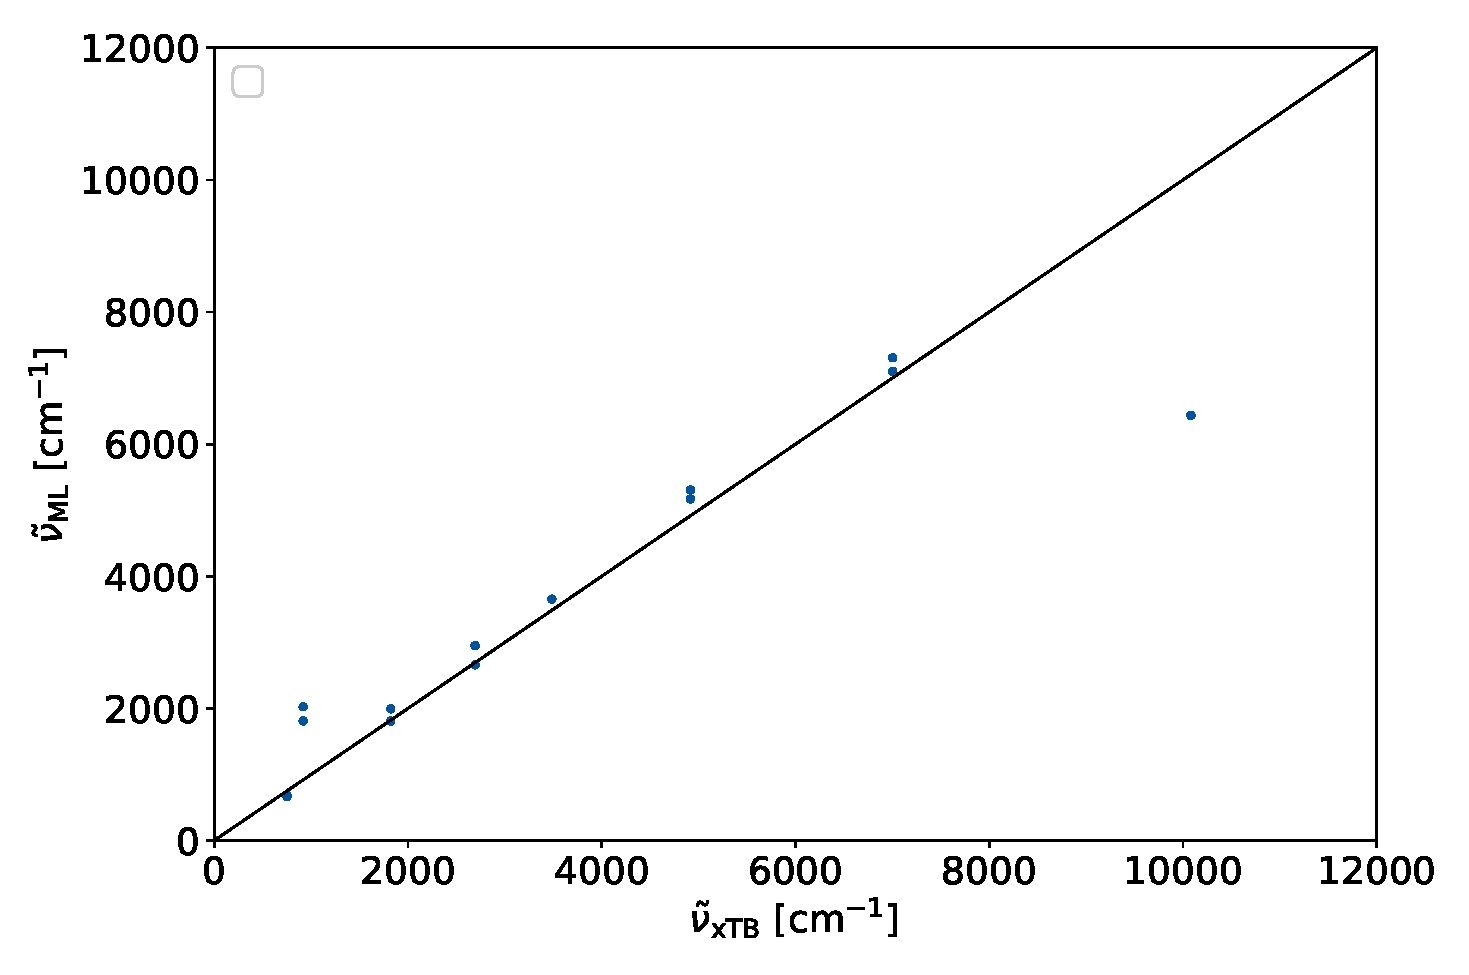
\includegraphics[width = \textwidth]{H2_single/Clean.eps}
    \caption[Plot of wavenumber from GFN2--xTB against wavenumber predicted by a ML model.]{ The wavenumber, predicted via the ML model $\tilde{\nu}_\mathrm{ML}$
    is plotted against the wavenumber calculated via GFN2--xTB $\tilde{\nu}_\mathrm{xTB}$.
    The model uses the Extra Tree Regression.
    The sample set is $\mathrm{H}_2$ and the training set is 75~\% of the whole set.
    The prediction were done for 5 random states.}
    \label{fig:WN_H2}
\end{figure}

\section{Comparison of RFR and ETF}
For the ML models two different algorithms were used, which are the ETR and RFR.
These models are compared to each other by testing there dependency on the amount of training set used.
As the quantity for testing the performance the MSE 
between the predicted hessian and the hessian computed via GFN2--xTB is used.\\
It is expected, that the performance of the ML model should increase, the more data it is trained with. 
To verify this behavior, the training set was increased successively.
The full training set is 75~\% of the full data set. Thus, test set is 25~\%.
While keeping the test set constant, the training set is changed successively between 7.5~\% of the data set to 75~\%.
The MSE was calculated for ten different random states and the mean of these MSE was calculated.
Fig~\ref{fig:Comparison_RFR_ETR} shows the MSE in the dependency of the amount of training set used for the ETR (on the left)
and the RFR (on the right). The error bars indicate the standard deviation.
\begin{figure}[H]
    \centering
    \subfloat{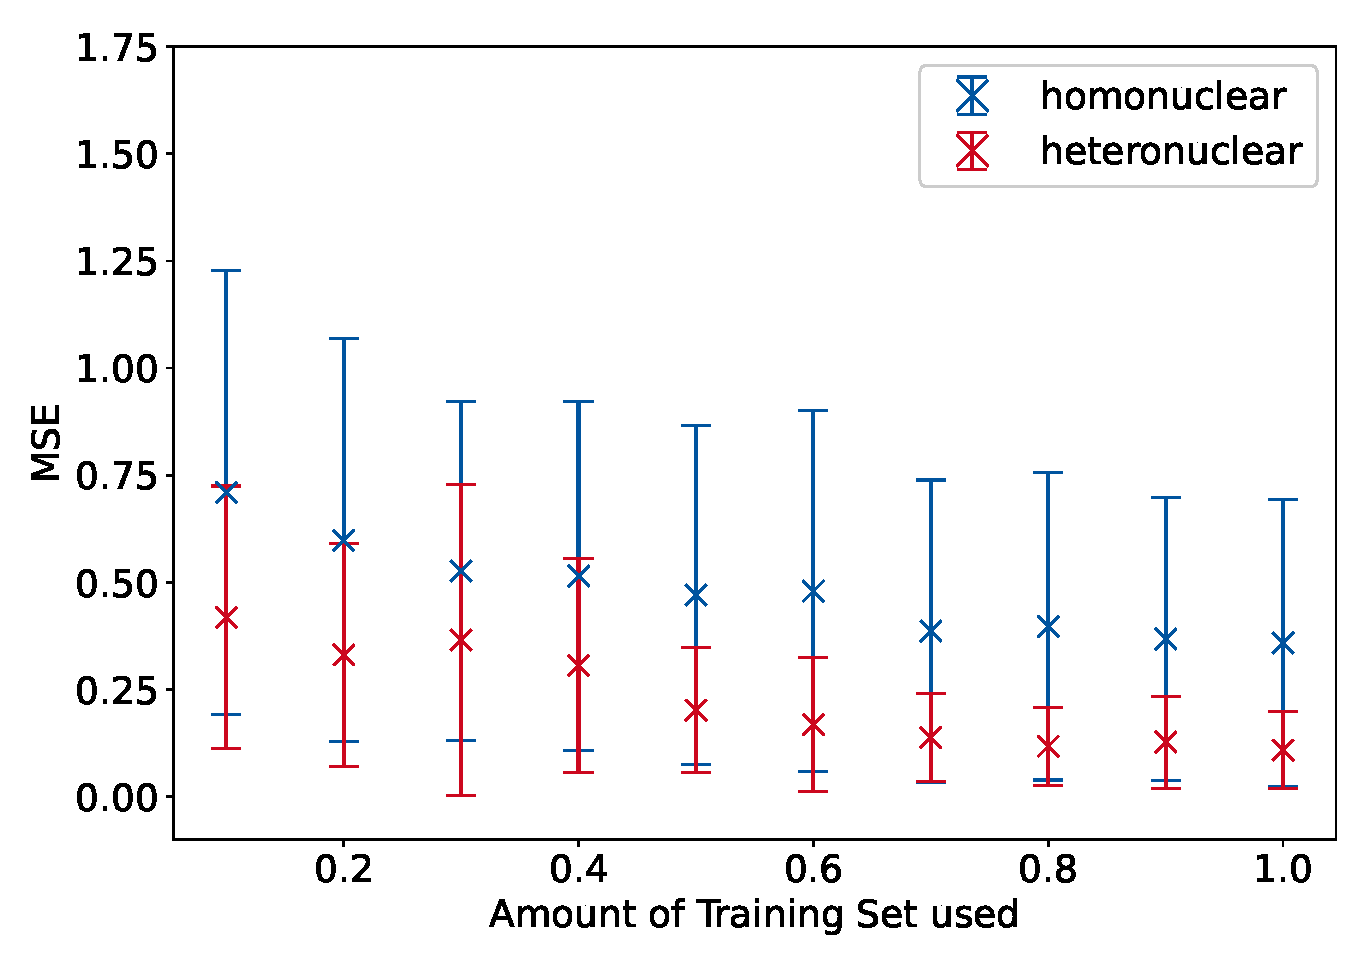
\includegraphics[width = 0.5\textwidth ]{MSE/MSE_ETR.eps}}
    \hfill
    \subfloat{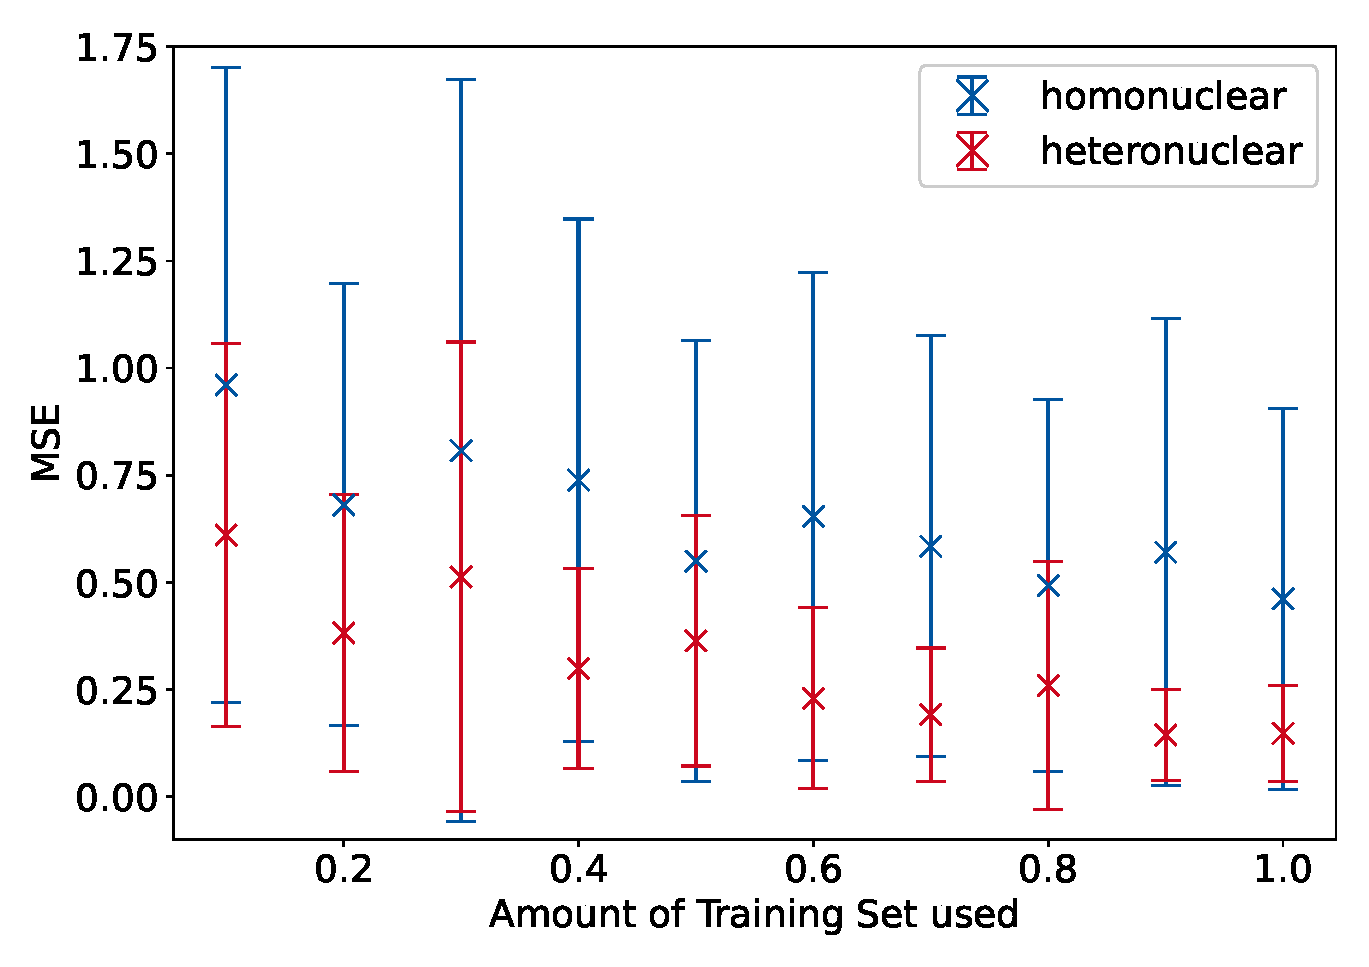
\includegraphics[width = 0.5\textwidth ]{MSE/MSE_RFR.eps}}
    \caption[Learning plots of the ETR and RFR for an increasing size of the training set]{
    Learning plots for the predicting hessian elements~$\frac{\partial^2H}{\partial a \partial b}$
    for an increase of the amount of training set used.
    On the left is the learning plot of the Extra Tree Regression and on the right the plot of the Random Forest Regression shown.
    The full training set is 75~\% of the sample set.
    The full sample set, excluding the $\mathrm{H}_3$~system, is used.
    The mean of ten random states were used for the MSE.
    The plots are done for the homonuclear model (blue) and heteronuclear model (red).}
    \label{fig:Comparison_RFR_ETR}
\end{figure}
In the case of the ETR, the MSE decreases with an increase of the amount of training set used for the homonuclear and heteronuclear model.
This behavior is also recognizable in the case of the RFR.
In comparison to the ETR, the RFR shows a higher standard deviation for the data points.
Thus, the RFR depends more strongly on the random state than the ETR. 
Furthermore, the ETR has, especially for the homonuclear model, lower MSE values for any amount of training set.
At the full amount of training set and at 90\% of the training set,
the RFR and ETR show a similar performance for the heteronuclear model.
All in all, the ETR shows a better performance for the whole investigated range.\\
There is the possibility, that the ML model has so much information in the features,
that it can always predict the target. Hence, the model is tested on whether this is the case,
or the ML model learns from the information of the feature.
For this, the features are scattered with a random factor.
The intensity of the scattering is amplified by the factor $\sigma$.
It is expected, that a model that learns from the features performs worse,
if the scattering of the data points increases.
\begin{figure}[H]
    \centering
    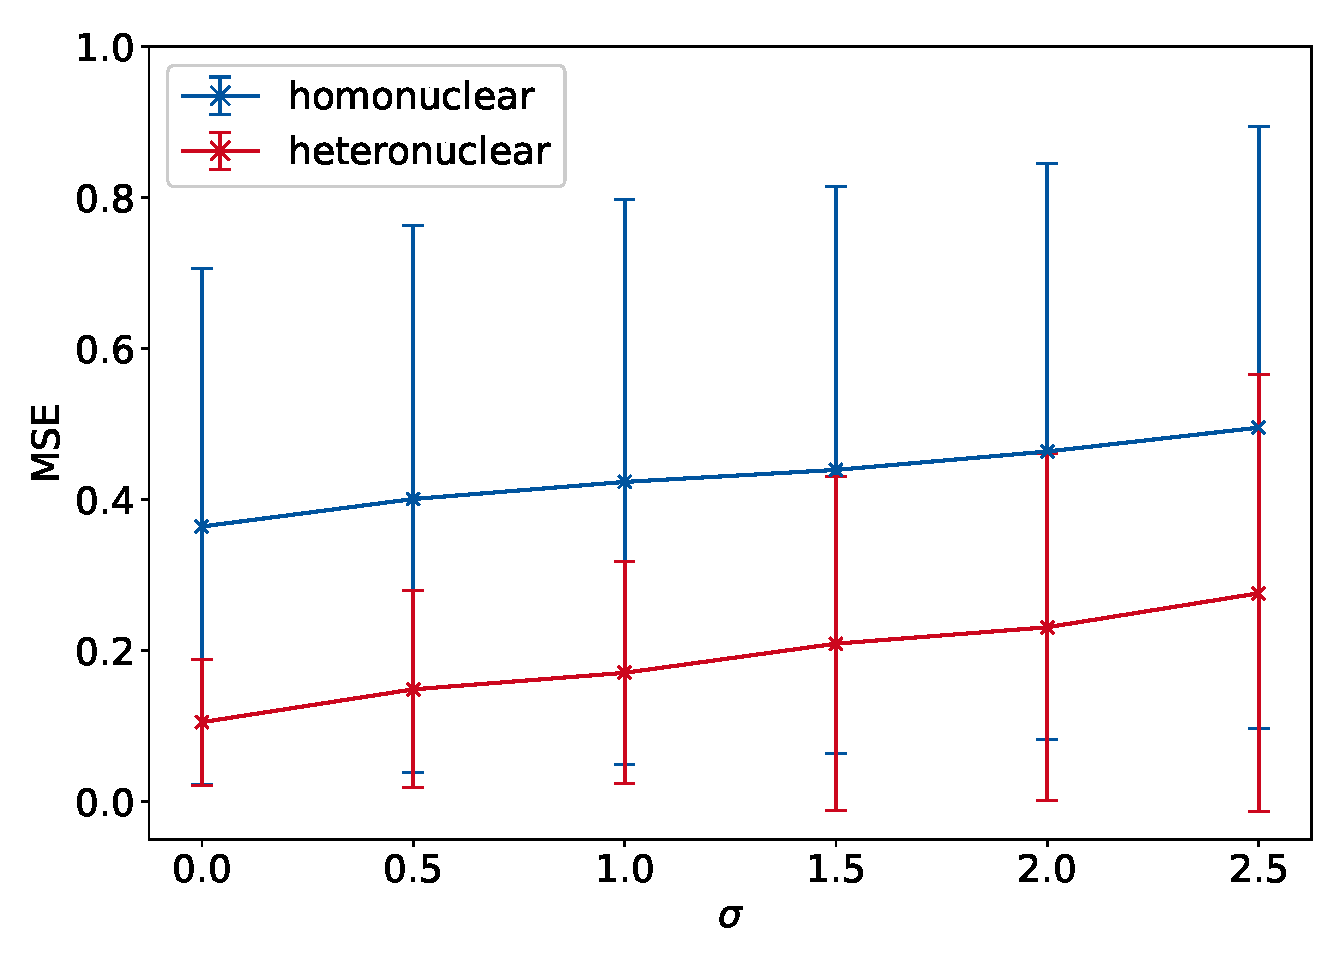
\includegraphics[width = \textwidth]{MSE/MSE_vs_sigma.eps}
    \caption[Learning plot for hessian elements with an increase of randomness on $\textbf{x}$]{
    Learning plots for predicting hessian elements~$\frac{\partial^2H}{\partial a \partial b}$
    for a variation of the factor~$\sigma$.
    The full sample set, excluding the $\mathrm{H}_3$~system, is used for the Ml models.
    The mean of ten random states were used for the MSE.
    The plots are done for the homonuclear model (blue) and heteronuclear model (red).}
    \label{fig:MSE_sigma}
\end{figure}
The performance of the model ETR--Multi--Permuted was tested for this. 
The prediction was done for ten different random states.
The MSE between the predicted hessian elements and the via GFN2--xTB calculated ones was investigated.
For the investigated range of $0 \leq \sigma \leq 2.5$ the MSE increases monotonically.
Hence, this shows, that the model learns from the features and is not purely random.\\
In this section a comparison of the RFR and ETR was done.
The ETR shows overall a better performance than the RFR.
Furthermore, it could be verified,
that the ML model learns from the features used for the prediction of the hessian matrices.


\section{Comparison of Permutation Model and Indexed Model}
Beside the different algorithms for the construction of the trees, other model changes were done.
These differences are investigated in this section. On the one hand,
a multimolecule model was constructed as also several single molecules.
On the other hand, it can be differentiated between the indexed and permuted model.
For the investigations in this section, 
the difference between the prediction and GFN2--xTB calculation were computed.
From these differences the standard deviation as also the mean were calculated,
and a Gaussian distribution was assumed.
This was done for the models ETR--Perm--Multi, ETR--Perm--Single, ETR--Idx--Multi and ETR--Idx--Single.\\
At first the direct prediction of the hessian elements were investigated.
Fig.~\ref{fig:ErrorDistHess} shows the distribution for the prediction of the hessian elements.

\begin{figure}[H]
    \centering
    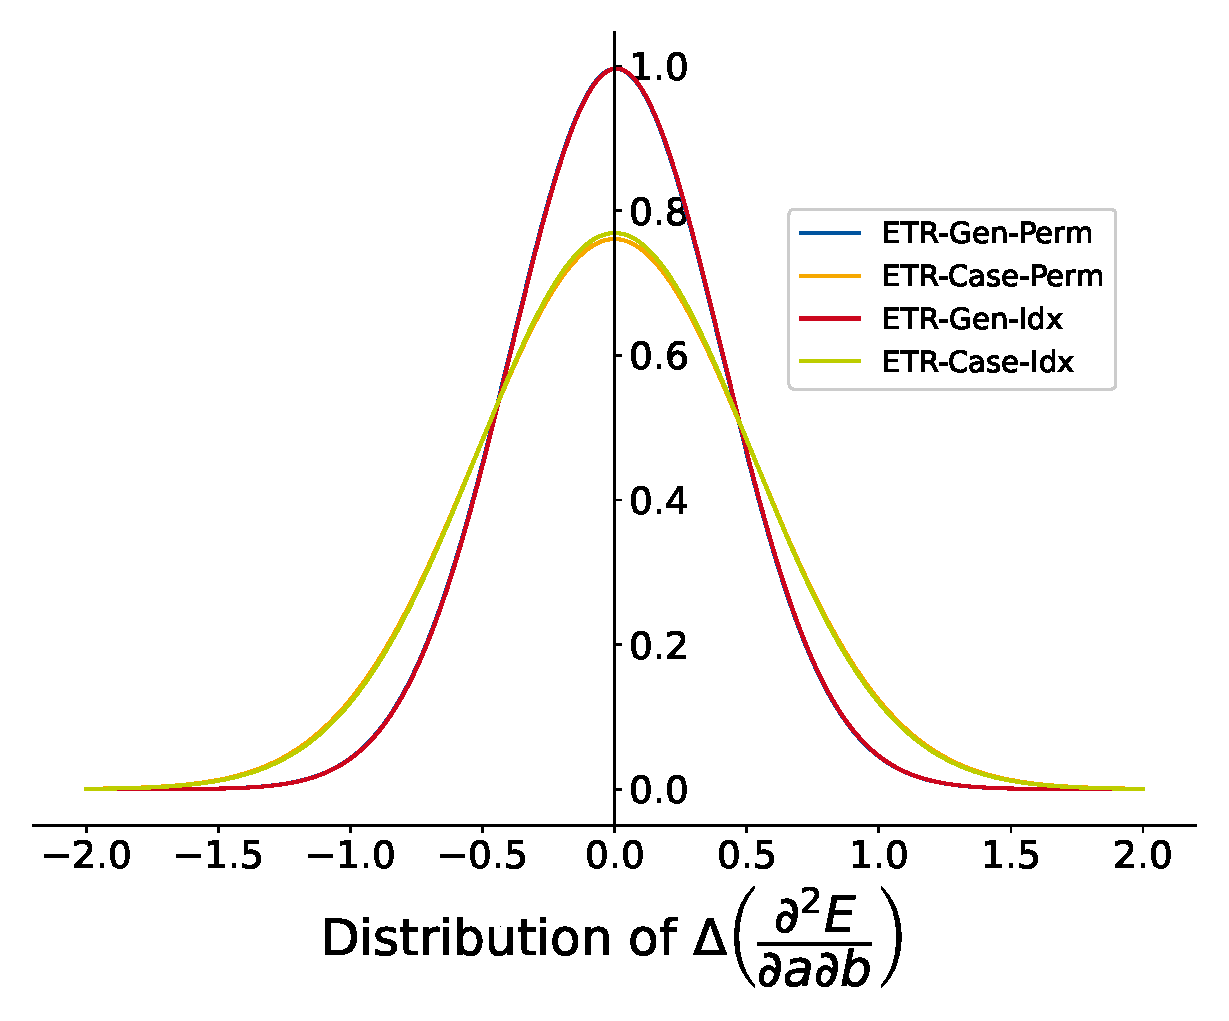
\includegraphics[width = \textwidth]{ErrorDistGraphs/error_distribution_ml_hess.eps}
    \caption[Gaussian type distribution for the prediction of hessian elements.]{ Distribution of $\Delta \left(\frac{\partial^2 E}{\partial a \partial b}\right)$ for different models.
    In every model, the Extra Tree Regression was used.
    The distribution is assumed to be Gaussian type.
    For this the median and standard deviation of $\Delta \left(\frac{\partial^2 E}{\partial a \partial b}\right)$ are computed. }
    \label{fig:ErrorDistHess}
\end{figure}
Comparing the ETR--Perm--Single and ETR--Idx--Single as also ETR--Perm--Multi and ETR--Idx--Multi shows,
that both approaches for the labeling of the features do not differ significantly.
Thus, both approaches are in good agreement with another.
This shows, on the one hand, the strength of the decision tree algorithms.
They cannot overfit and seem to be capable of describing this complex system with a simple differentiation by indexes.
On the other hand, the permuted model does the same prediction for the model,
but may be useful for other machine learning algorithms or even neural networks.\\
The comparison of the ETR--Perm--Single and ETR--Perm--Multi
shows, that the ETR--Perm--Single model deviates more strongly.
This is in agreement with the comparison of the ETR--Idx--Single and ETR--Idx--Multi models.
Though the deviation is stronger, the means of the models do not differ significantly. 
The data set for training the models is smaller for the Single models than for the Multi models.
This might be the reason for the deviation.\\

\begin{figure}[H]
    \centering
    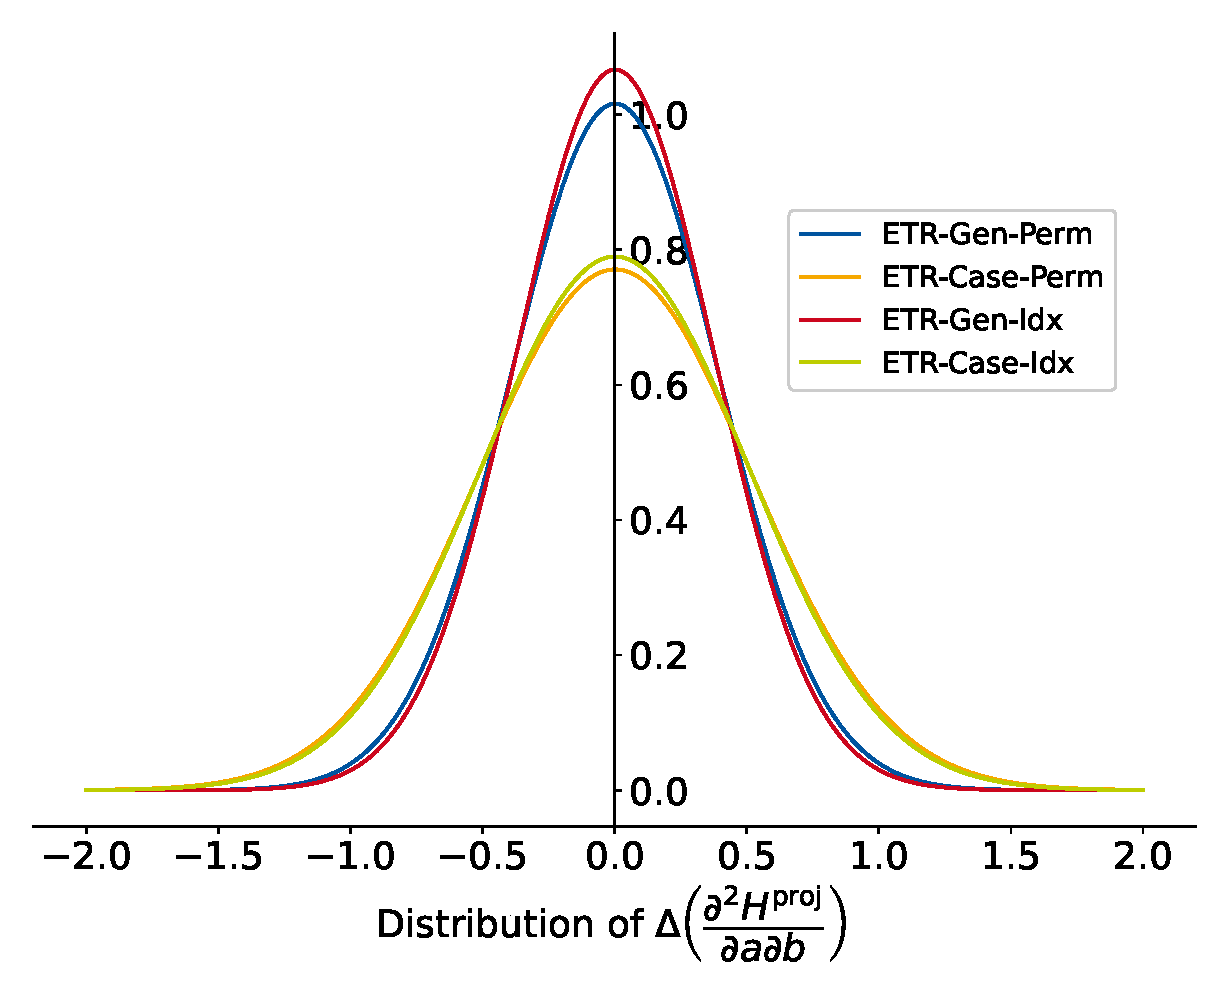
\includegraphics[width = \textwidth]{ErrorDistGraphs/error_distribution_ml_hess_p.eps}
    \caption[Gaussian type distribution for the prediction of projected hessian elements.]{
    Distribution of $\Delta \left(\frac{\partial^2 E^\mathrm{proj}}{\partial a \partial b}\right)$ for different models.
    In every model, the Extra Tree Regression was used.
    The distribution is assumed to be Gaussian type.
    For this the median and standard deviation of $\Delta \left(\frac{\partial^2 E^\mathrm{proj}}{\partial a \partial b}\right)$ are computed. }
    \label{fig:ErrorDistHessP}
\end{figure}

\begin{figure}[H]
    \centering
    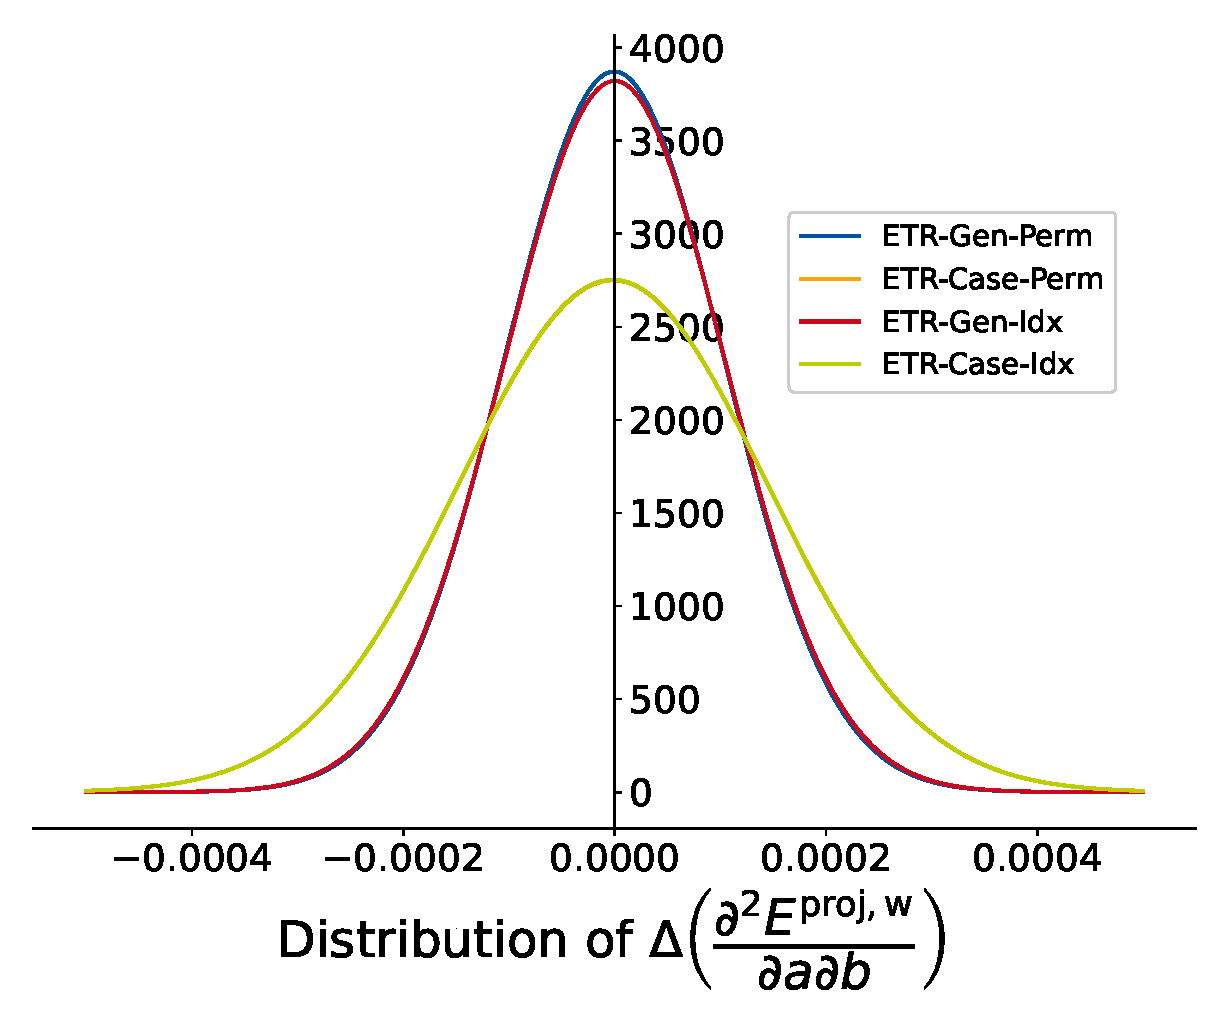
\includegraphics[width = \textwidth]{ErrorDistGraphs/error_distribution_ml_hess_w.eps}
    \caption[Gaussian type distribution for the prediction of weighted projected hessian elements.]{
    Distribution of $\Delta \left(\frac{\partial^2 E^\mathrm{proj,w}}{\partial a \partial b}\right)$ for different models.
    In every model, the Extra Tree Regression was used.
    The distribution is assumed to be Gaussian type.
    For this the median and standard deviation of $\Delta \left(\frac{\partial^2 E^\mathrm{proj,w}}{\partial a \partial b}\right)$ are computed. }    \label{fig:ErrorDistHessW}
\end{figure}

\begin{figure}[H]
    \centering
    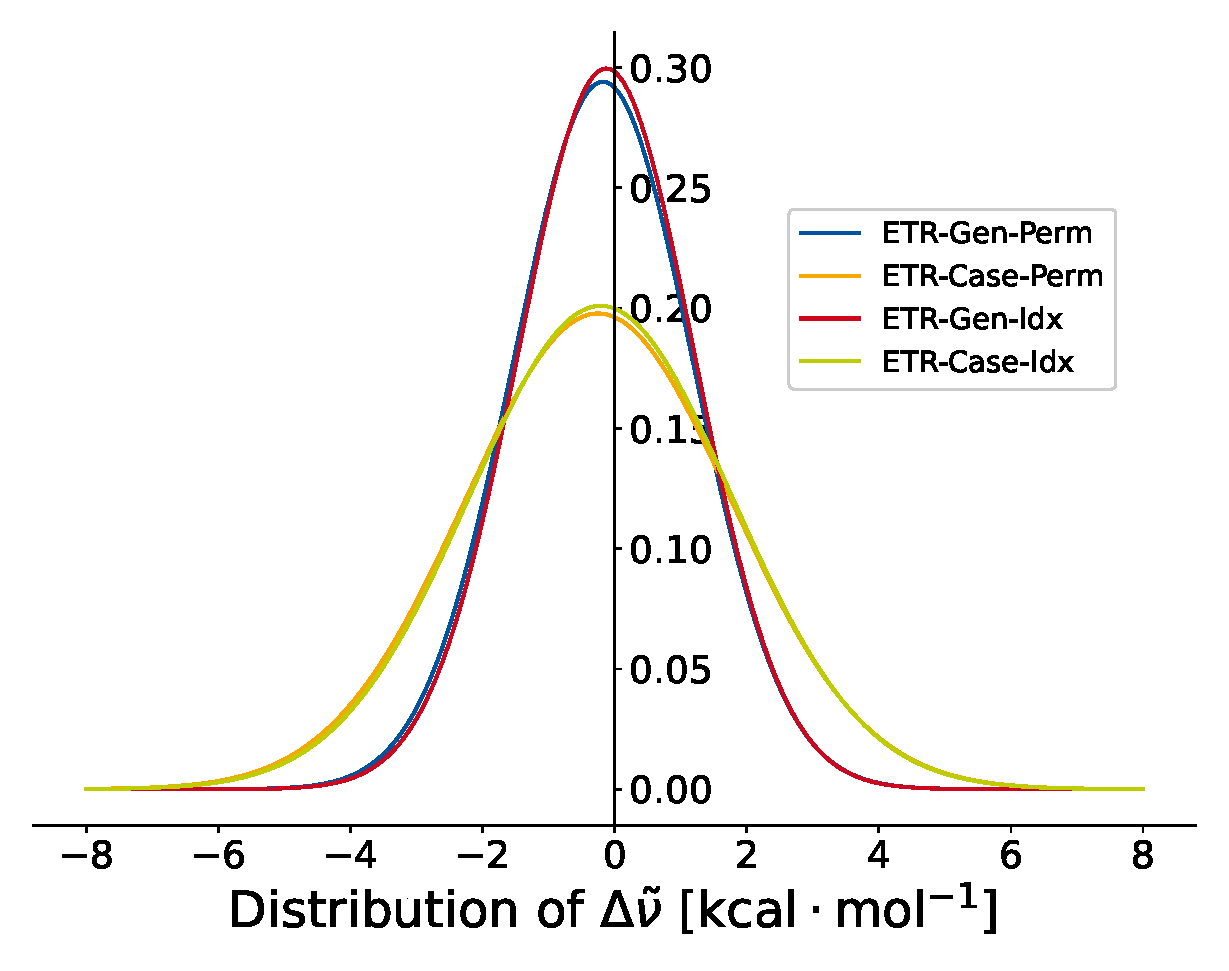
\includegraphics[width = \textwidth]{ErrorDistGraphs/error_distribution_ml_wn.eps}
    \caption[Gaussian type distribution for the prediction of wavenumbers.]{
    Distribution of $\Delta \tilde{\nu}$ for different models.
    In every model, the Extra Tree Regression was used.
    The distribution is assumed to be Gaussian type.
    For this the median and standard deviation of $\Delta \tilde{\nu}$ are computed.}
    \label{fig:ErrorDistWN}
\end{figure}

\begin{figure}[H]
    \centering
    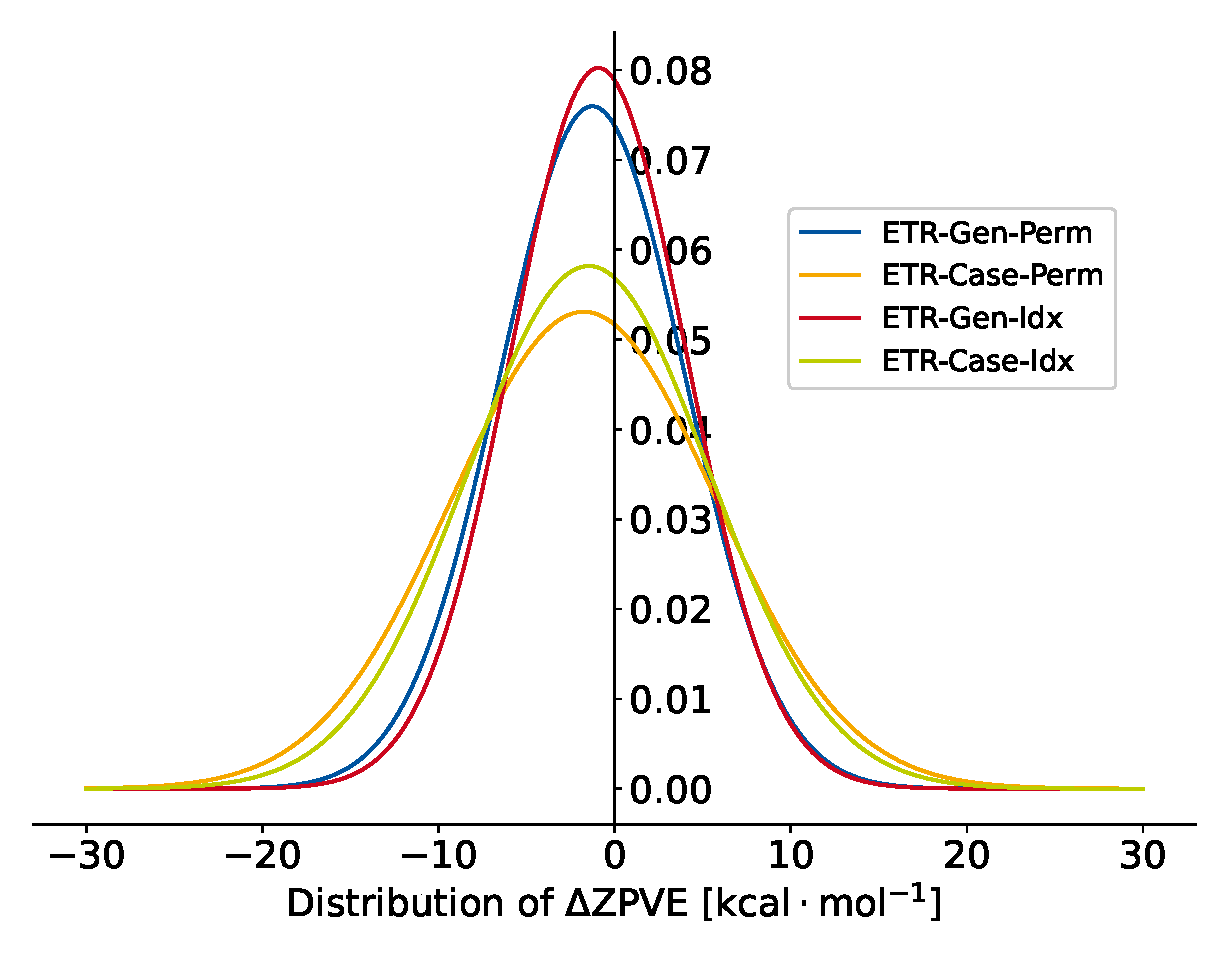
\includegraphics[width = \textwidth]{ErrorDistGraphs/error_distribution_ml_ZPE.eps}
    \caption[Gaussian type distribution for the prediction of zero point energy.]
    {Distribution of $\Delta \mathrm{ZPE}$ for different models.
    In every model, the Extra Tree Regression was used.
    The distribution is assumed to be Gaussian type.
    For this the median and standard deviation of $\Delta \mathrm{ZPE}$ are computed.}
    \label{fig:ErrorDistZPE}
\end{figure}

\section{Benchmarking the H$_\mathrm{\textbf{3}}$~system}
Especially, the prediction of hessian matrices of fully unknown systems is of interest.
Hence, the ETR-Gen-Perm and ETR-Gen-Idx models were tested on the performance on a new, for the model unknown, system.
For the $\mathrm{H}_3$ system the outer hydrogen atoms were fixed,
while the hydrogen atom was shift from one hydrogen to another.
For each position of the hydrogen atom,
the force constants of the systems were predict via the ML model.
The force constants were also calculated via GFN2--xTB.\\
Fig.~\ref{fig:FC_idx} shows the force constants calculated by GFN2--xTB and predicted via the ETR--Gen--Idx model.
Interesting to point out is the symmetric behavior of the system.
The ML model should, in principle, mimic this behavior.
While this is overall the case, there are abbreviation from this behavior.
For the example, the symmetry is not given in the case of $x(\mathrm{H2}) = 1.75$ and $x(\mathrm{H2} = 2.25)$.
\begin{figure}[H]
    \centering
    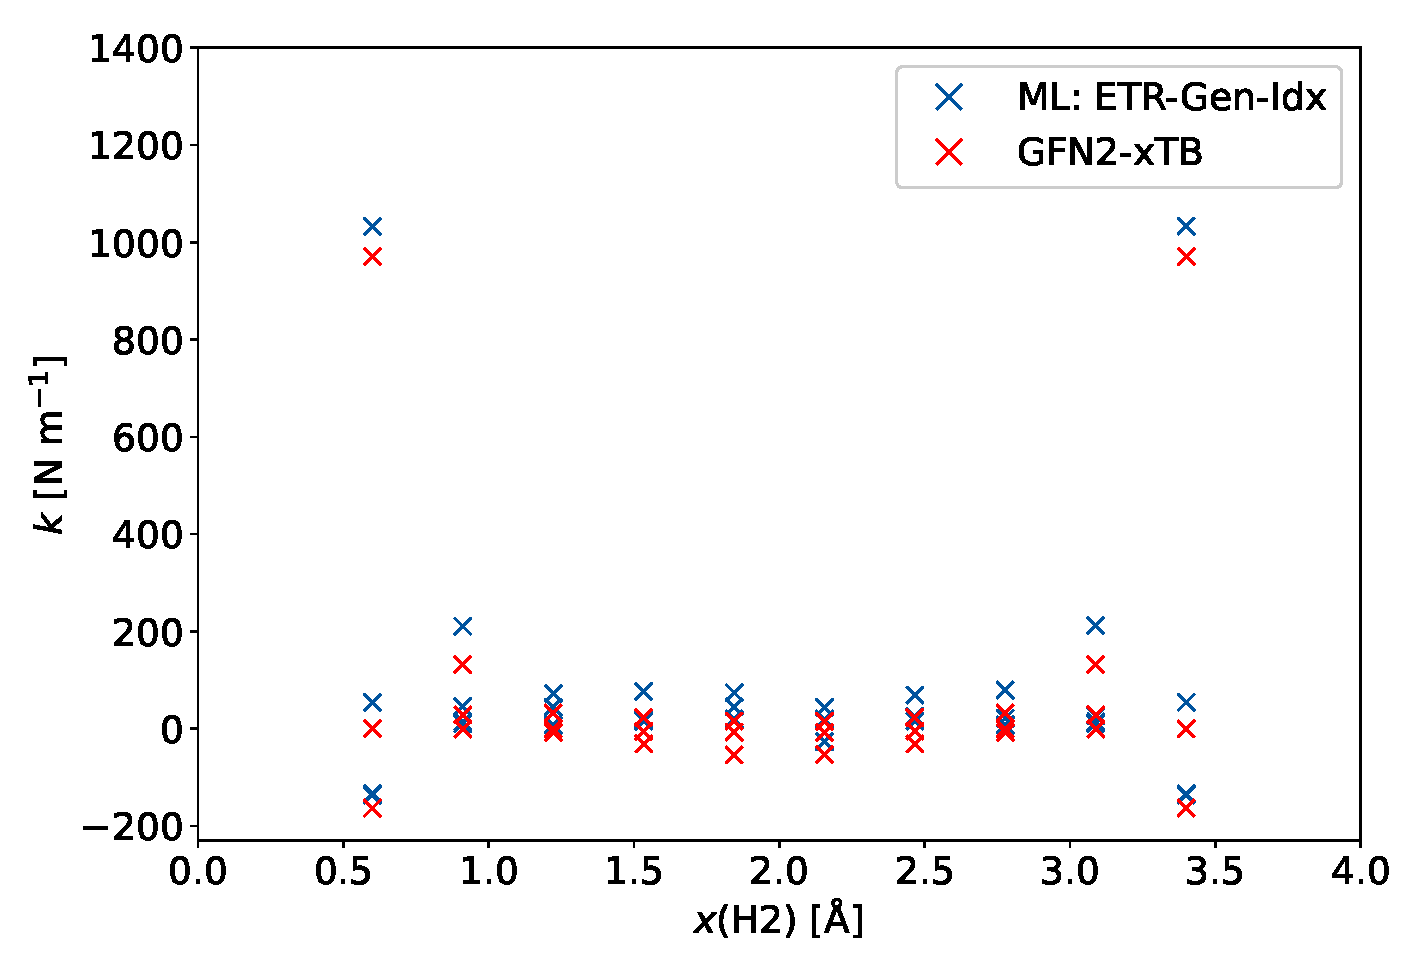
\includegraphics[width = \textwidth]{ForceConstants/force_const_H3_idx.eps}
    \caption[Force constants predicted by the indexed multimodel and calculated with
    GFN2--xTB for $\mathrm{H}_3$~system]{
    Force constants predicted for the $\mathrm{H}_3$~systems in dependence of the distance between H1 and H2 are shown.
    The force constants are shown for the GFN2--xTB calculation (yellow),
    as also the via the ML model predicted values (blue).
    The full sample set, excluding the $\mathrm{H}_3$~system, was used for the ML model.
    The ML model \textit{indexed; multi} was used for the prediction.
    }
    \label{fig:FC_idx}
\end{figure}

\begin{figure}[H]
    \centering
    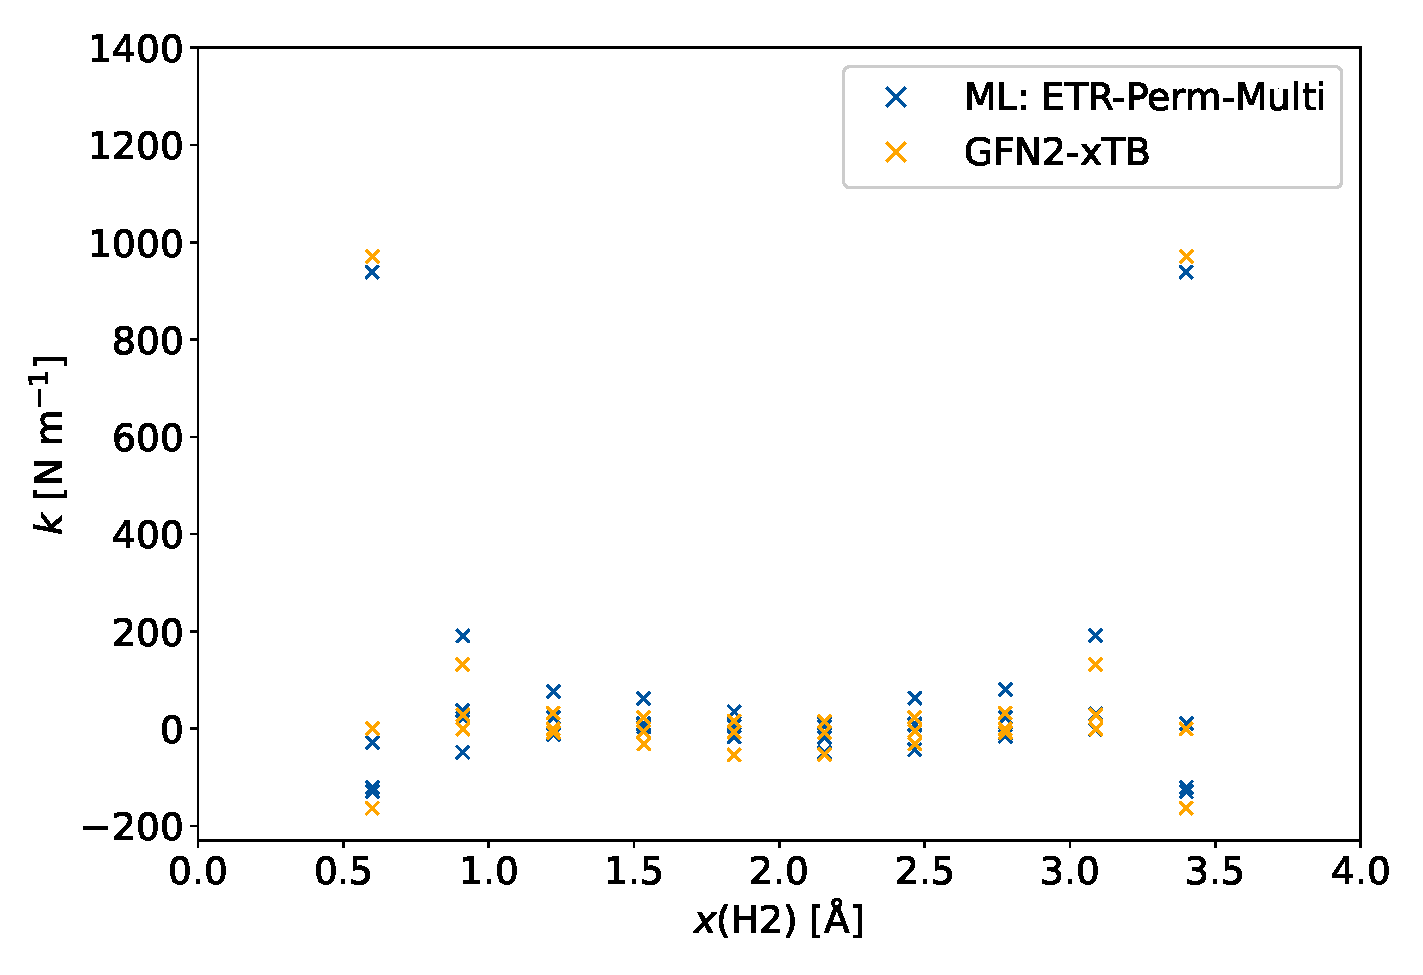
\includegraphics[width = \textwidth]{ForceConstants/force_const_H3_perm.eps}
    \caption[Force constants predicted by the permuted multimodel and calculated with
    GFN2--xTB for $\mathrm{H}_3$~system]{Force constants predicted for the $\mathrm{H}_3$~systems in dependence of the distance between H1 and H2 are shown.
    The force constants are shown for the GFN2--xTB calculation (yellow),
    as also the via the ML model predicted values (blue).
    The full sample set, excluding the $\mathrm{H}_3$~system, was used for the ML model.
    The ML model \textit{perm; multi} was used for the prediction.}
    \label{fig:FC_perm}
\end{figure}


	\newpage
	\chapter{Bibliography}
	\begingroup
	\renewcommand{\chapter}[2]{}
	
	\printbibliography
	\endgroup

	\newpage
	\chapter{Appendix}

\begin{subequations}
    \label{eq:Feature}
\begin{align}
    CN_A &= \sum_{B \neq A}^{N_\mathrm{atoms}} \dfrac{1}{1+\exp\left(\dfrac{-16a\cdot 4 (R_{A,\mathrm{cov}}+R_{B,\mathrm{cov}})}{3R_{AB}-1}\right)} \\
    CN^\mathrm{ext} &= \sum_{B \neq A}^{N_\mathrm{atoms}} \dfrac{CN_B}{f_\mathrm{damp}(R_A,R_B)}\\
    q_A &= Zg_A - \sum_{\mu \in A}^{N_\mathrm{BF}}\sum_{\nu}^{N_\mathrm{BF}} P_{\mu \nu} S_{\mu \nu}\\
    q_A^\mathrm{ext} &= q_A + \sum_{B \neq A}^{N_\mathrm{atoms}} \dfrac{q_B}{f_\mathrm{damp}}\\
    \mu_A^\alpha &= \sum_{l\in A} \sum_{\kappa \in l \in A} \sum_{\lambda} P_{\kappa \lambda}\left(\alpha_A S_{\lambda \kappa} - D_{\lambda \kappa}^{\alpha}\right)\\
    \mu_A^{\alpha,\mathrm{ext}} &= \mu_A^{\alpha} + \sum_{B \neq A} \dfrac{\mu_B^\alpha - \alpha_{AB} q_B}{f_\mathrm{damp} \cdot (CN_B + 1)}\\
    \mathrm{with}&:~\alpha_{AB} = \alpha_A - \alpha_B\\
    \mu_{A,p}^{\alpha,\mathrm{ext}} &= \mu_A^\alpha + \sum_{B \neq A} \dfrac{\mu_B^\alpha+ \alpha_{AB} p_B}{f_\mathrm{damp} (CN_B+1)}\\
    \theta_A^{\alpha \beta} &=   \sum_{l \in A} \dfrac{3}{2}\Theta_l^{\alpha \beta} - \dfrac{\delta^{\alpha \beta}}{2} (\Theta^{xx}_l + \Theta^{yy}_l +\Theta^{zz}_l) \\
    \mathrm{with}&:~\Theta_l^{\alpha \beta} = \sum_{\kappa \in l \in A} \sum_A P_{\kappa \lambda} \left(\alpha_A D_{\lambda \kappa}^\beta +\beta_A D_{\lambda \kappa}^\alpha - \alpha_A \beta_A S_{\lambda \kappa } - Q_{\lambda \kappa}^{\alpha \beta}\right) \nonumber \\
    \mathrm{and}&:~\delta^{\alpha \beta}=\begin{cases}
     1~\mathrm{if}: \alpha = \beta \\
     0~\mathrm{if}: \alpha \neq \beta\\   
    \end{cases} \nonumber \\
    \bm{\uptheta}_A &= \left(\begin{matrix}
        \theta_A^{\mathrm{xx}} & \theta_A^{\mathrm{xy}} & \theta_A^{\mathrm{xz}} \\
        \theta_A^{\mathrm{xy}} & \theta_A^{\mathrm{yy}} & \theta_A^{\mathrm{yz}} \\
        \theta_A^{\mathrm{xz}} & \theta_A^{\mathrm{yz}} & \theta_A^{\mathrm{yz}} \\
    \end{matrix}\right) \times \textbf{1}\\
    \theta_A^{\mathrm{ext},\alpha \beta} &= \theta_A^{\alpha \beta} + \dfrac{\theta^{\alpha \beta}_B + \delta \theta^{\alpha \beta}_B}{f_\mathrm{damp}(CN_B+1) }\\
    \bm{\uptheta}_A^\mathrm{ext} &= \left(\begin{matrix}
        \theta_A^{\mathrm{ext,xx}} & \theta_A^{\mathrm{ext,xy}} & \theta_A^{\mathrm{ext,xz}} \\
        \theta_A^{\mathrm{ext,xy}} & \theta_A^{\mathrm{ext,yy}} & \theta_A^{\mathrm{ext,yz}} \\
        \theta_A^{\mathrm{ext,xz}} & \theta_A^{\mathrm{ext,yz}} & \theta_A^{\mathrm{ext,yz}} \\
    \end{matrix}\right) \times \textbf{1}
\end{align}

\begin{align}
    E_{A,\mathrm{EHT}} &= \sum_{k \in A} \sum_k P_{k\lambda} H_{k\lambda}\\
    E_{A,\mathrm{rep}} &= \sum_{B \neq A}^{M} \dfrac{1}{2} \dfrac{Y_{A}^\mathrm{eff}Y_{B}^\mathrm{eff}}{R_{AB}}
    \cdot \exp \left(\alpha_A \alpha_B \right)^{0.5} R_{AB}^{k_\mathrm{rep}}\\
    E_{A,\mathrm{disp}}^{(2)} &= \sum_{A \neq B} \sum_{n=6,8} -s_n \dfrac{1}{2}
    \dfrac{C_n^{AB}(q_a,CN_\mathrm{cov}^A,q_b,CN_\mathrm{cov}^B)}{R_{AB}^n} f_{n}^\mathrm{damp,BJ}(R_{AB})\\
    E_{A,\mathrm{disp}}^{(3)} &= \sum_{B \neq A} \sum_{C \neq B \neq A} 
    -s_9 \dfrac{1}{3} 
    \dfrac{(3 \cos(\theta_{ABC}) \cos(\theta_{BCA} \cos(\theta_{CBA}) + 1))}{(R_{AB}R_{AC}R_{BC})^3} \nonumber\\ 
    &\cdot  C_9^{ABC}(CN_\mathrm{cov}^A,CN_\mathrm{cov}^B,CN_\mathrm{cov}^C) \cdot 
    f_{9}^\mathrm{damp,zero}(R_{AB},R_{AC},R_{BC})\\
    E_{A,\mathrm{AES}} &= E_{A,q\mu} + E_{A,q\theta} + E_{A,\mu\mu} \nonumber \\
    &= \sum_{B \neq A} \dfrac{1}{2} \bigg(f_3(R_{AB})\big[q_A(\bm{\mu}_B^\intercal\textbf{R}_{BA}) + q_B (\bm{\upmu}_A^\intercal)\textbf{R}_{AB} \big] \nonumber\\
    &+ f_5(R_{AB}) \big[q_A\bm{R}_{BA}^\intercal \bm{\Uptheta}_B \bm{R}_{BA} +q_B\bm{R}_{BA}^\intercal \bm{\Uptheta}_A \bm{R}_{BA} \nonumber \\
    &- 3 (\bm{\upmu}_A^\intercal\bm{R}_{AB})(\bm{\upmu}_B^\intercal\bm{R}_{AB}) +  (\bm{\upmu}_A^\intercal \bm{\upmu}_B R_{AB}^2)  \big] \bigg)\\
    E_{A,\mathrm{AXS}} &= \left( f_\mathrm{XC}^{\mu_A}|\bm{\upmu}_A|^2  + f_\mathrm{XC}^{\Theta_A}||\bm{\Uptheta}_A||^2  \right) \\
    E_{A,\mathrm{IES+IXC}} &= \dfrac{1}{2} \sum_{B \neq A} \sum_{l \in A} \sum_{l' \in B} q_{A,l} q_{B,l'} \gamma_{AB,ll'} + \dfrac{1}{3} \sum_{l \in A} \Gamma_{A,l} q_{A,l}^3
\end{align}
\end{subequations}

\begin{table}[H]
    \centering
    \caption[List of indices used for the differentiation of Hessian elements.]{Indices used for the different elements in a Hessian matrix block to differ between the elements.}
        \begin{tabular}{c c c c | c }
            \hline
            & &  Indexed& & Permuted \\
            Hessian element &  $x^\mathrm{idx}$ & $y^\mathrm{idx}$ & $z^\mathrm{idx}$ & Index\\
            \hline
            \\[-1em]
            $\dfrac{\partial^2 E}{\partial x_A \partial x_B}$ & 2 & 0 & 0 & 0\\
            \\[-1em]
            $\dfrac{\partial^2 E}{\partial x_A \partial y_B}$ & 1 & -1 &  0 & 1\\
            \\[-1em] 
            $\dfrac{\partial^2 E}{\partial x_A \partial z_B}$ & 1 & 0 &  -1 & 2\\
            \\[-1em]
            $\dfrac{\partial^2 E}{\partial y_A \partial x_B}$ & -1 & 1 &  0 & 1\\
            \\[-1em]
            $\dfrac{\partial^2 E}{\partial y_A \partial y_B}$ & 0 & 2 &  0 & 0\\
            \\[-1em]
            $\dfrac{\partial^2 E}{\partial y_A \partial z_B}$ & 0 & 1 &  -1 & 2\\
            \\[-1em]
            $\dfrac{\partial^2 E}{\partial z_A \partial x_B}$ & -1 & 0 &  1 & 2\\
            \\[-1em]
            $\dfrac{\partial^2 E}{\partial z_A \partial y_B}$ & 0 & -1 &  1 & 2\\
            \\[-1em]
            $\dfrac{\partial^2 E}{\partial z_A \partial z_B}$ & 0 & 0 &  2 & 3\\
            \\[-1em]
            \hline 
        \end{tabular}
    \label{tab:Indices}
\end{table}

\begin{table}[H]
    \centering
    \caption[]{Permutation of the coordinates for each Hessian element.
    At first the permutation of the vectors is shown.
    After that, the change of the elements of a matrix, for example, for the quadrupole moment is shown.}
        \begin{tabular}{c c c c c c c c c c}
            \hline\\[-1em]
            Hessian &\\
            &$\dfrac{\partial^2 E}{\partial x_A \partial x_A}$ & $\dfrac{\partial^2 E}{\partial x_A \partial y_A}$ &
            $\dfrac{\partial^2 E}{\partial x_A \partial z_A}$ &$\dfrac{\partial^2 E}{\partial y_A \partial x_A}$ &
            $\dfrac{\partial^2 E}{\partial y_A \partial y_A}$ &$\dfrac{\partial^2 E}{\partial y_A \partial z_A}$ &
            $\dfrac{\partial^2 E}{\partial z_A \partial x_A}$ & $\dfrac{\partial^2 E}{\partial z_A \partial y_A}$ &
            $\dfrac{\partial^2 E}{\partial z_A \partial z_A}$ \\[+0.7em]
            \hline
            Vector\\
            x &  x  &  y    & z  & x   &y   & z     &x     & y  & z\\ 
            y &  y  &  x    & x  & y   & z  & y     & z    & z  & x \\
            z &  z  & $-$z  & y  & z   &x   &$-$x   & $-$y & x  & y\\
            \hline 
            Matrix\\
            xx & xx & yy    & zz & xx  & yy & zz    & xx   & yy & zz \\
            yy & xy & xx    & xx & yy  & zz & yy    & zz   & zz & xx \\
            zz & xz & zz    & yy & zz  & xx & xx    & yy   & xx & yy \\
            xy & xy & xy    & xz & xy  & yz & yz    & xz   & yz & xz \\
            xz & xz & $-$yz & yz & xz  & xy & $-$xz & $-$xy& xy & yz \\
            yz & yz & $-$xz & xy & yz  & xz & $-$xy & $-$yz& xz & xy \\
            \hline 
        \end{tabular}
    \label{tab:Permutation}
\end{table}


\begin{figure}[H]
    \hspace*{-0.25cm}
    \subfloat[homonuclear model]
    {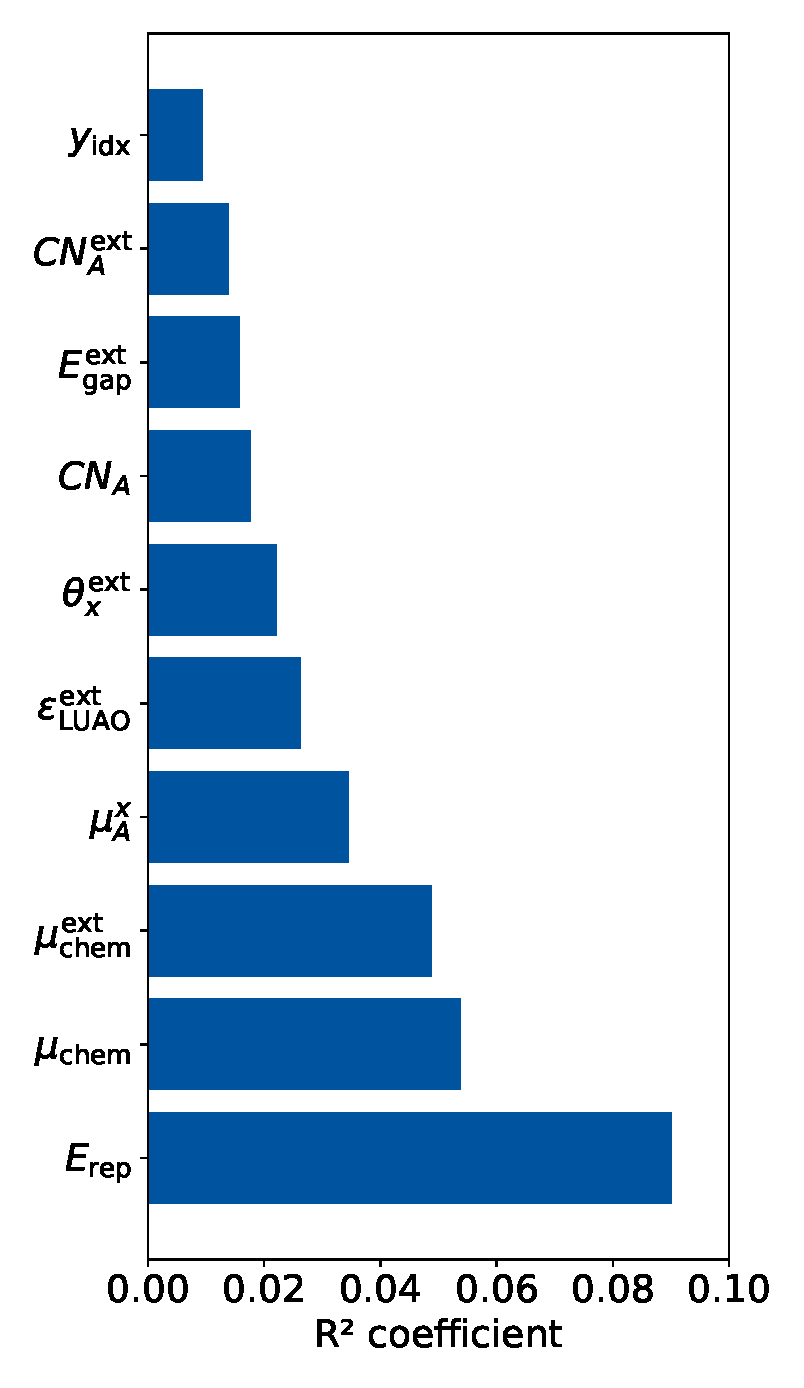
\includegraphics[width = 0.48\textwidth]{PearsonCorrelationCoeffiecient/PCC_diag_perm.eps}}
    \hspace*{0.25cm}
    \subfloat[heteronuclear model]{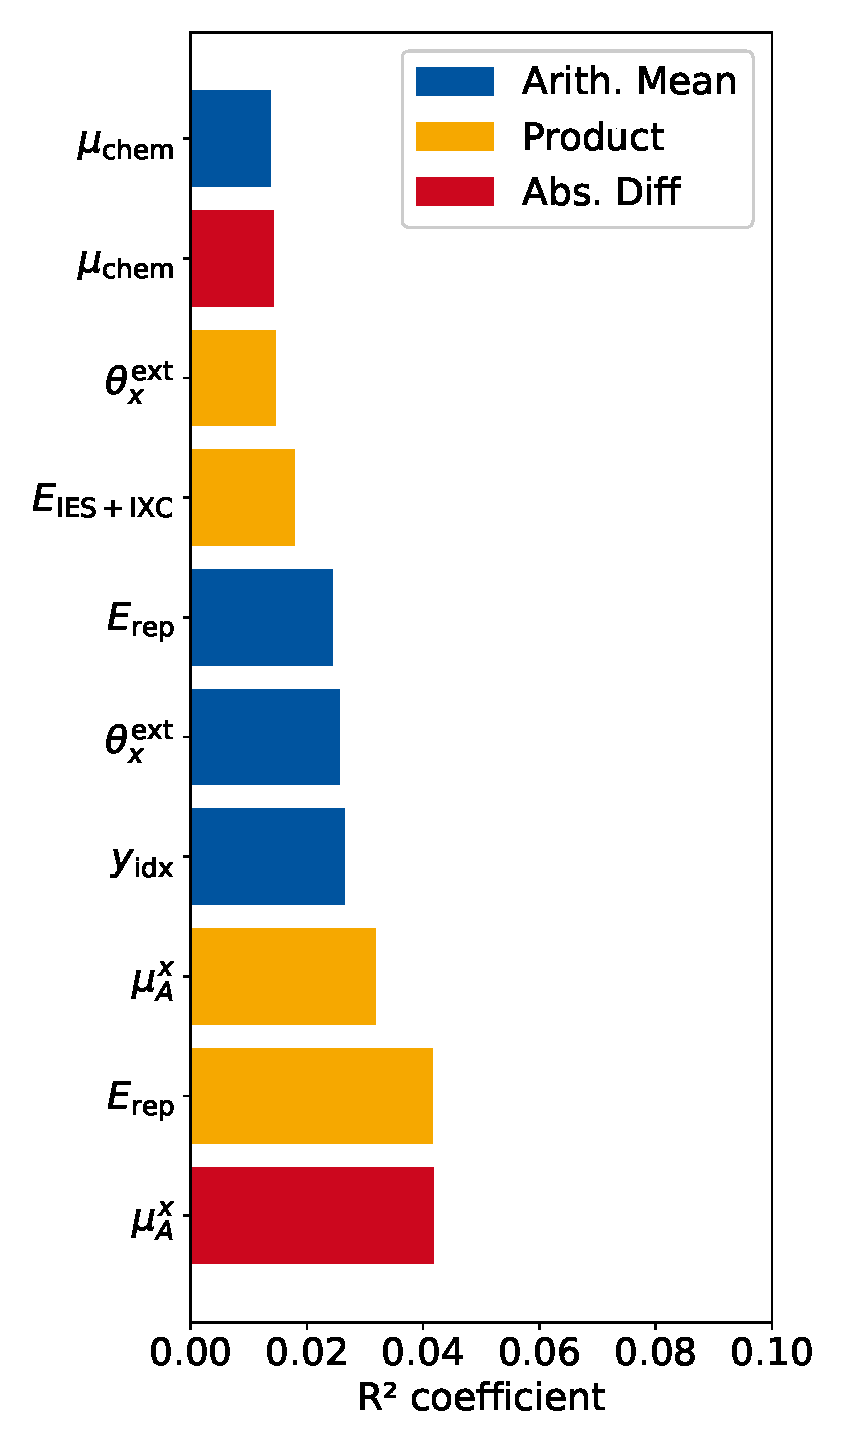
\includegraphics[width = 0.48\textwidth]{PearsonCorrelationCoeffiecient/PCC_ndiag_perm.eps}}
    \caption[Pearson Correlation Coefficient for the ten most important features (Gen--Perm model).]{
                Pearson Correlation Coefficient for the features used for the homonuclear and heteronuclear model.
                The ten features with the highest coefficients are shown for each model.
                The features are constructed with the Gen--Perm model.
                }
    \label{fig:PCC_perm}
\end{figure}

\begin{figure}[H]
    \hspace*{-0.25cm}
    \subfloat[homonuclear model]
    {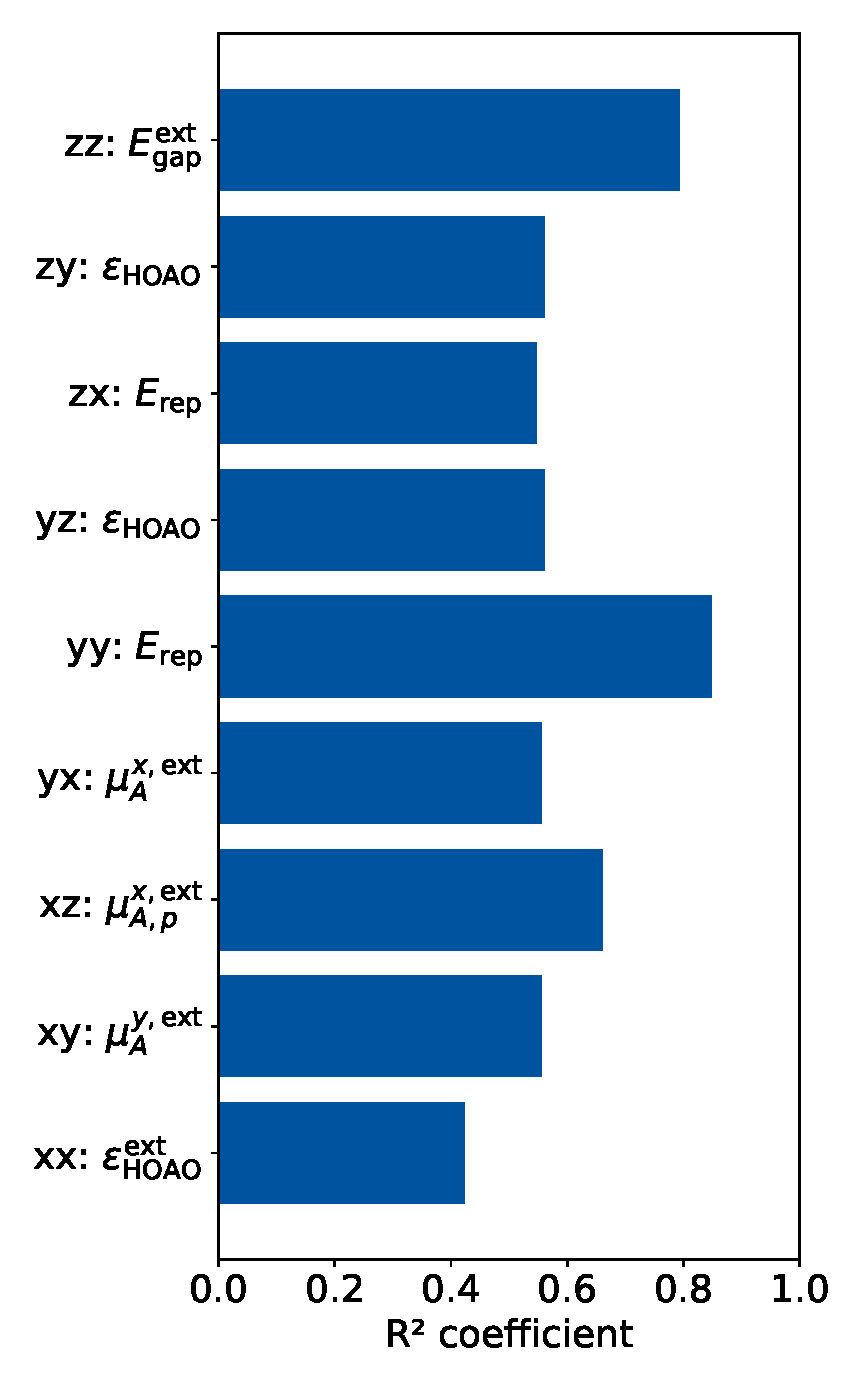
\includegraphics[width = 0.48\textwidth]{PearsonCorrelationCoeffiecient/PCC_element_specific_diag_perm.eps}}
    \hspace*{0.25cm}
    \subfloat[heteronuclear model]{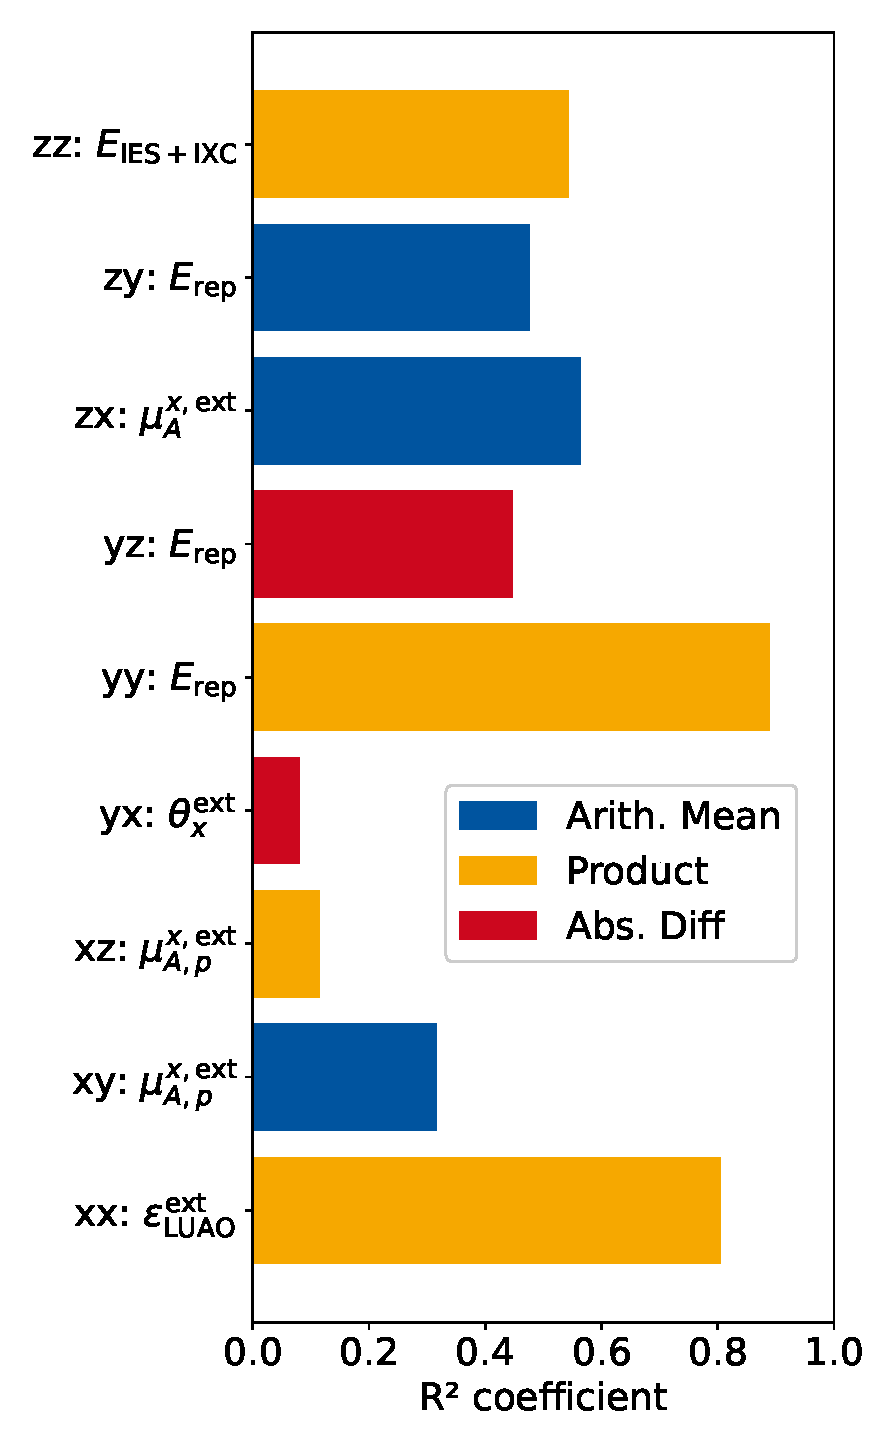
\includegraphics[width = 0.48\textwidth]{PearsonCorrelationCoeffiecient/PCC_element_specific_nondiag_perm.eps}}
    \caption[Best Pearson Correlation Coefficient computed element wise (Gen--Perm model).]{
        Highest Pearson Correlation Coefficient specifically computed for each Hessian element for the homo-- and heteronuclear model.
        The abbreviation ab corresponds to the elements $\frac{\partial^2 E}{\partial a_A \partial b_B}$.
        The features are constructed with the Gen--Perm model.
                }
    \label{fig:PCC_elementwise_Perm}
\end{figure}

\begin{figure}[H]
    \centering
    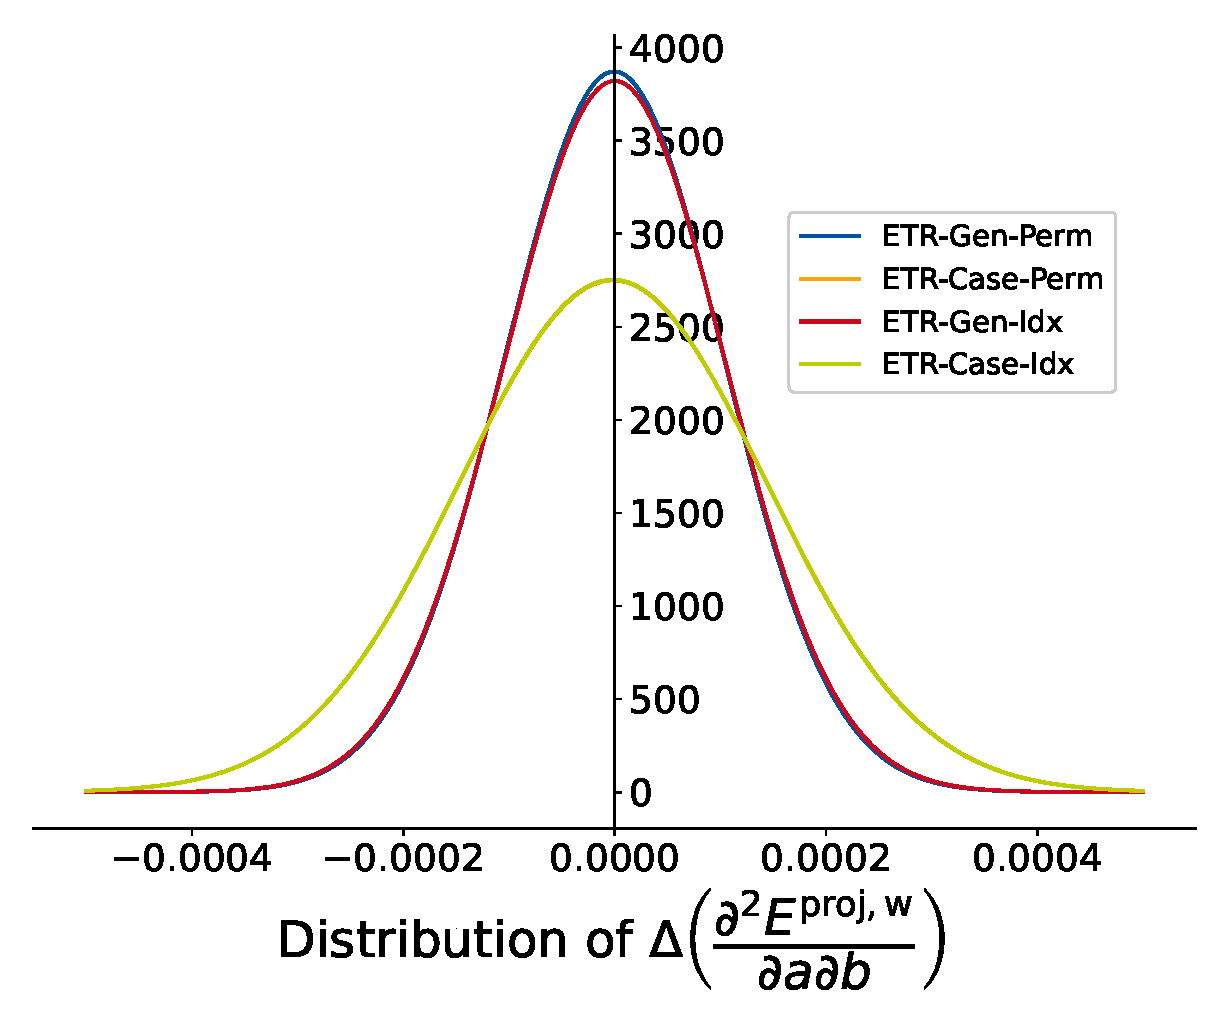
\includegraphics[width = \textwidth]{ErrorDistGraphs/error_distribution_ml_hess_w.eps}
    \caption[Gaussian type distribution for the prediction of weighted projected Hessian elements.]{
    Distribution of $\Delta \left(\frac{\partial^2 E^\mathrm{proj,w}}{\partial a \partial b}\right)$ for different models.
    In every model, the ETR was used.
    A Gaussian distribution is assumed.
    For this the median and standard deviation of $\Delta \left(\frac{\partial^2 E^\mathrm{proj,w}}{\partial a \partial b}\right)$ are computed. }    \label{fig:ErrorDistHessW}
\end{figure}

\begin{figure}[H]
    \centering
    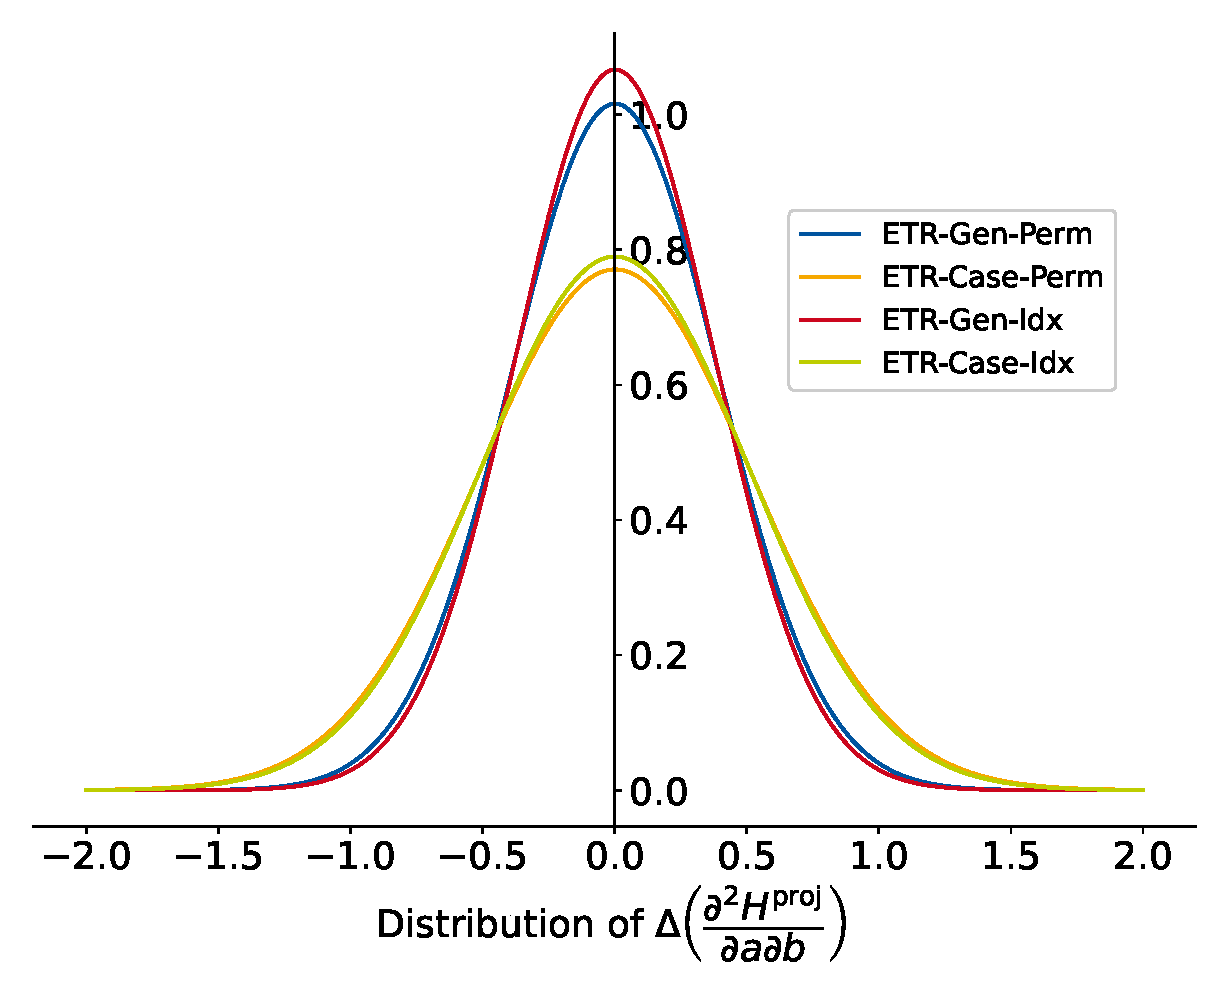
\includegraphics[width = \textwidth]{ErrorDistGraphs/error_distribution_ml_hess_p.eps}
    \caption[Gaussian type distribution for the prediction of projected Hessian elements.]{
    Distribution of $\Delta \left(\frac{\partial^2 E^\mathrm{proj}}{\partial a \partial b}\right)$ for different models.
    In every model, the ETR was used.
    A Gaussian distribution is assumed.
    For this the median and standard deviation of $\Delta \left(\frac{\partial^2 E^\mathrm{proj}}{\partial a \partial b}\right)$ are computed. }
    \label{fig:ErrorDistHessP}
\end{figure}
    
\begin{figure}[H]
    \centering
    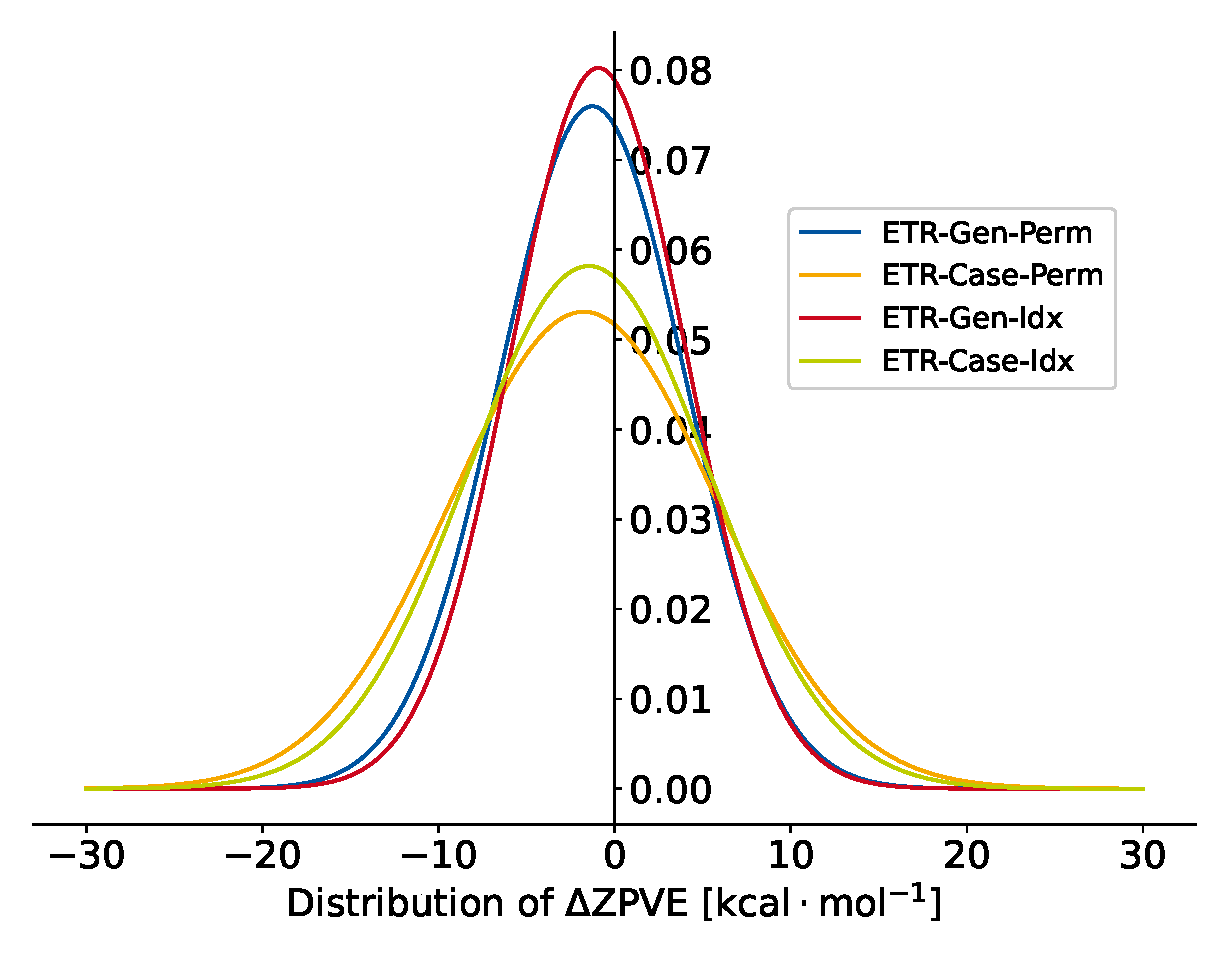
\includegraphics[width = \textwidth]{ErrorDistGraphs/error_distribution_ml_ZPE.eps}
    \caption[Gaussian type distribution for the prediction of zero point energy.]
    {Distribution of $\Delta \mathrm{ZPE}$ for different models.
    In every model, the ETR was used.
    A Gaussian distribution is assumed.
    For this the median and standard deviation of $\Delta \mathrm{ZPE}$ are computed.}
    \label{fig:ErrorDistZPE}
\end{figure}

	%\begin{figure}[H]
	%	\centering
	%	\includegraphics[width = \textwidth]{Figures/cutoff_convergence_full.eps}
	%	\caption{full cutoff}
	%	\label{fig:cutoff_full}
	%\end{figure}
	%\begin{figure}[H]
	%	\centering
	%	\includegraphics[width = \textwidth]{Figures/kpt_convergence_full.eps}
	%	\caption{full kpt}
	%	\label{fig:kpts_full}
	%\end{figure}
	
	%\begin{figure}[H]
	%	\centering
	%	\includegraphics[width = \textwidth]{Figures/E_vs_Dist_Layer.pdf}
	%	\caption{Energy vs Distance for adsorption on surface with 1,2,3 layers of atoms}
	%	\label{fig:E_dist}
	%\end{figure}
\end{document}